% **************************************************************************************************************
% A Classic Thesis Style
% An Homage to The Elements of Typographic Style
%
% Copyright (C) 2015 André Miede http://www.miede.de
%
% If you like the style then I would appreciate a postcard. My address 
% can be found in the file ClassicThesis.pdf. A collection of the 
% postcards I received so far is available online at 
% http://postcards.miede.de
%
% License:
% This program is free software; you can redistribute it and/or modify
% it under the terms of the GNU General Public License as published by
% the Free Software Foundation; either version 2 of the License, or
% (at your option) any later version.
%
% This program is distributed in the hope that it will be useful,
% but WITHOUT ANY WARRANTY; without even the implied warranty of
% MERCHANTABILITY or FITNESS FOR A PARTICULAR PURPOSE.  See the
% GNU General Public License for more details.
%
% You should have received a copy of the GNU General Public License
% along with this program; see the file COPYING.  If not, write to
% the Free Software Foundation, Inc., 59 Temple Place - Suite 330,
% Boston, MA 02111-1307, USA.
%
% **************************************************************************************************************

\RequirePackage{fix-cm} % fix some latex issues see: http://texdoc.net/texmf-dist/doc/latex/base/fixltx2e.pdf

\documentclass[ twoside,openright,titlepage,numbers=noenddot,headinclude,%1headlines,% letterpaper a4paper
                footinclude=true,cleardoublepage=empty,abstractoff, % <--- obsolete, remove (todo)
                BCOR=5mm,paper=a4,fontsize=11pt,%11pt,a4paper,%
                ngerman,american,%
                ]{scrreprt}

\usepackage[utf8]{inputenc}	
\usepackage{etoolbox}


%% ---------------------------------------------------------------------------------------------------------------------

\newcommand{\myTitle}{Collide, Collate, Collect: Decoding Wireless Collisions\xspace}
\newcommand{\myDegree}{Bachelor Thesis\xspace}
\newcommand{\myName}{Johannes Lauinger\xspace}
\newcommand{\myProf}{Prof. Dr.-Ing. Matthias Hollick\xspace}
\newcommand{\mySupervisor}{Robin Klose M.Sc.\xspace}
\newcommand{\myThesiscode}{SEEMOO-BSC-$0000$\xspace} % You will get this from your supervisor
\newcommand{\myFaculty}{Department of Computer Science\xspace}
\newcommand{\myDepartment}{Secure Mobile Networking Lab\xspace}
\newcommand{\myUni}{\protect{Technische Universität Darmstadt}\xspace}
\newcommand{\myLocation}{Darmstadt\xspace}
\newcommand{\myTime}{\formatdate{01}{08}{2017}\xspace}
\newcommand{\myVersion}{0.1\xspace}


% Choose if you want the standard template with enough space for margin notes or the tempate with small margins
\newtoggle{adrianstyle}
\toggletrue{adrianstyle}    % uncomment this line to have smaller margins
%\togglefalse{adrianstyle}  % uncomment this line for the standard seemoo template


% ****************************************************************************************************
% classicthesis-config.tex 
% formerly known as loadpackages.sty, classicthesis-ldpkg.sty, and classicthesis-preamble.sty 
% Use it at the beginning of your ClassicThesis.tex, or as a LaTeX Preamble 
% in your ClassicThesis.{tex,lyx} with % ****************************************************************************************************
% classicthesis-config.tex 
% formerly known as loadpackages.sty, classicthesis-ldpkg.sty, and classicthesis-preamble.sty 
% Use it at the beginning of your ClassicThesis.tex, or as a LaTeX Preamble 
% in your ClassicThesis.{tex,lyx} with % ****************************************************************************************************
% classicthesis-config.tex 
% formerly known as loadpackages.sty, classicthesis-ldpkg.sty, and classicthesis-preamble.sty 
% Use it at the beginning of your ClassicThesis.tex, or as a LaTeX Preamble 
% in your ClassicThesis.{tex,lyx} with \input{classicthesis-config}
% ****************************************************************************************************  
% If you like the classicthesis, then I would appreciate a postcard. 
% My address can be found in the file ClassicThesis.pdf. A collection 
% of the postcards I received so far is available online at 
% http://postcards.miede.de
% ****************************************************************************************************

% ****************************************************************************************************
% 1. Configure classicthesis for your needs here, e.g., remove "drafting" below 
% in order to deactivate the time-stamp on the pages
% ****************************************************************************************************
\PassOptionsToPackage{eulerchapternumbers,listings,%
                 %drafting,%
				 pdfspacing,%floatperchapter,%linedheaders,%
				 subfig,beramono,eulermath,parts,dottedtoc,%
				 \iftoggle{adrianstyle}{adrianstyle}{}, % Use this option to increase the text width
				 }{classicthesis}								
% ********************************************************************
% Available options for classicthesis.sty 
% (see ClassicThesis.pdf for more information):
% drafting
% parts nochapters linedheaders
% eulerchapternumbers beramono eulermath pdfspacing minionprospacing
% tocaligned dottedtoc manychapters
% listings floatperchapter subfig
% ********************************************************************


% ****************************************************************************************************
% 2. Loading some handy packages
% ****************************************************************************************************
%\PassOptionsToPackage{spanish,es-lcroman}{babel}

% ********************************************************************
% Setup, finetuning, and useful commands
% ********************************************************************
\newcounter{dummy} % necessary for correct hyperlinks (to index, bib, etc.)
\newlength{\abcd} % for ab..z string length calculation
% ****************************************************************************************************


% ****************************************************************************************************
% 3. Loading some handy packages
% ****************************************************************************************************
% ******************************************************************** 
% Packages with options that might require adjustments
% ******************************************************************** 
%\PassOptionsToPackage{ngerman,american}{babel}   % change this to your language(s)
% Spanish languages need extra options in order to work with this template
%\PassOptionsToPackage{spanish,es-lcroman}{babel}
	\usepackage{babel}                  

\usepackage{csquotes}
\PassOptionsToPackage{%
    %backend=biber, %instead of bibtex
	backend=bibtex8,bibencoding=ascii,%
	language=auto,%
	style=numeric-comp,%
    %style=authoryear-comp, % Author 1999, 2010
    %bibstyle=authoryear,dashed=false, % dashed: substitute rep. author with ---
    sorting=nyt, % name, year, title
    maxbibnames=10, % default: 3, et al.
    %backref=true,%
    natbib=true % natbib compatibility mode (\citep and \citet still work)
}{biblatex}
    \usepackage{biblatex}

\PassOptionsToPackage{fleqn}{amsmath}       % math environments and more by the AMS 
    \usepackage{amsmath}

% ******************************************************************** 
% General useful packages
% ******************************************************************** 
\PassOptionsToPackage{T1}{fontenc} % T2A for cyrillics
    \usepackage{fontenc}     
\usepackage{textcomp} % fix warning with missing font shapes
\usepackage{scrhack} % fix warnings when using KOMA with listings package          
\usepackage{xspace} % to get the spacing after macros right  
\usepackage{mparhack} % get marginpar right
\usepackage{fixltx2e} % fixes some LaTeX stuff --> since 2015 in the LaTeX kernel (see below)
%\usepackage[latest]{latexrelease} % will be used once available in more distributions (ISSUE #107)
\usepackage[nopostdot,acronym,shortcuts,nonumberlist]{glossaries}
\makeglossaries
\renewcommand*{\glossarysection}[2][]{}
\input{acronyms.tex}
% ****************************************************************************************************


% ****************************************************************************************************
% 4. Setup floats: tables, (sub)figures, and captions
% ****************************************************************************************************
\usepackage{tabularx} % better tables
    \setlength{\extrarowheight}{3pt} % increase table row height
\newcommand{\tableheadline}[1]{\multicolumn{1}{c}{\spacedlowsmallcaps{#1}}}
\newcommand{\myfloatalign}{\centering} % to be used with each float for alignment
\usepackage{caption}
% Thanks to cgnieder and Claus Lahiri
% http://tex.stackexchange.com/questions/69349/spacedlowsmallcaps-in-caption-label
% [REMOVED DUE TO OTHER PROBLEMS, SEE ISSUE #82]    
%\DeclareCaptionLabelFormat{smallcaps}{\bothIfFirst{#1}{~}\MakeTextLowercase{\textsc{#2}}}
%\captionsetup{font=small,labelformat=smallcaps} % format=hang,
\captionsetup{font=small} % format=hang,
\usepackage{subfig}  
% ****************************************************************************************************


% ****************************************************************************************************
% 5. Setup code listings
% ****************************************************************************************************
\usepackage{listings} 
%\lstset{emph={trueIndex,root},emphstyle=\color{BlueViolet}}%\underbar} % for special keywords
\lstset{language=[LaTeX]Tex,%C++,
    morekeywords={PassOptionsToPackage,selectlanguage},
    keywordstyle=\color{RoyalBlue},%\bfseries,
    basicstyle=\small\ttfamily,
    %identifierstyle=\color{NavyBlue},
    commentstyle=\color{Green}\ttfamily,
    stringstyle=\rmfamily,
    numbers=none,%left,%
    numberstyle=\scriptsize,%\tiny
    stepnumber=5,
    numbersep=8pt,
    showstringspaces=false,
    breaklines=true,
    %frameround=ftff,
    %frame=single,
    belowcaptionskip=.75\baselineskip
    %frame=L
} 
% ****************************************************************************************************    		   


% ****************************************************************************************************
% 6. PDFLaTeX, hyperreferences and citation backreferences
% ****************************************************************************************************
% ********************************************************************
% Using PDFLaTeX
% ********************************************************************
\PassOptionsToPackage{pdftex,hyperfootnotes=false,pdfpagelabels}{hyperref}
    \usepackage{hyperref}  % backref linktocpage pagebackref
\pdfcompresslevel=9
\pdfadjustspacing=1 
\PassOptionsToPackage{pdftex}{graphicx}
    \usepackage{graphicx} 
 

% ********************************************************************
% Hyperreferences
% ********************************************************************
\hypersetup{%
    %draft,	% = no hyperlinking at all (useful in b/w printouts)
    %colorlinks=true, linktocpage=true, pdfstartpage=3, pdfstartview=FitV,%
    % uncomment the following line if you want to have black links (e.g., for printing)
    colorlinks=false, linktocpage=false, pdfborder={0 0 0}, pdfstartpage=3, pdfstartview=FitV,% 
    breaklinks=true, pdfpagemode=UseNone, pageanchor=true, pdfpagemode=UseOutlines,%
    plainpages=false, bookmarksnumbered, bookmarksopen=true, bookmarksopenlevel=1,%
    hypertexnames=true, pdfhighlight=/O,%nesting=true,%frenchlinks,%
    urlcolor=webbrown, linkcolor=RoyalBlue, citecolor=webgreen, %pagecolor=RoyalBlue,%
    %urlcolor=Black, linkcolor=Black, citecolor=Black, %pagecolor=Black,%
    pdftitle={\myTitle},%
    pdfauthor={\textcopyright\ \myName, \myUni, \myFaculty},%
    pdfsubject={},%
    pdfkeywords={},%
    pdfcreator={pdfLaTeX},%
    pdfproducer={LaTeX with hyperref and classicthesis}%
}

\pdfinfo{
   /CreationDate (D:20130424083342)
   /ModDate (D:20130424083342)
}

% ********************************************************************
% Setup autoreferences
% ********************************************************************
% There are some issues regarding autorefnames
% http://www.ureader.de/msg/136221647.aspx
% http://www.tex.ac.uk/cgi-bin/texfaq2html?label=latexwords
% you have to redefine the makros for the 
% language you use, e.g., american, ngerman
% (as chosen when loading babel/AtBeginDocument)
% ********************************************************************
\makeatletter
\@ifpackageloaded{babel}%
    {%
       \addto\extrasamerican{%
			\renewcommand*{\figureautorefname}{Figure}%
			\renewcommand*{\tableautorefname}{Table}%
			\renewcommand*{\partautorefname}{Part}%
			\renewcommand*{\chapterautorefname}{Chapter}%
			\renewcommand*{\sectionautorefname}{Section}%
			\renewcommand*{\subsectionautorefname}{Section}%
			\renewcommand*{\subsubsectionautorefname}{Section}%     
                }%
       \addto\extrasngerman{% 
			\renewcommand*{\paragraphautorefname}{Absatz}%
			\renewcommand*{\subparagraphautorefname}{Unterabsatz}%
			\renewcommand*{\footnoteautorefname}{Fu\"snote}%
			\renewcommand*{\FancyVerbLineautorefname}{Zeile}%
			\renewcommand*{\theoremautorefname}{Theorem}%
			\renewcommand*{\appendixautorefname}{Anhang}%
			\renewcommand*{\equationautorefname}{Gleichung}%        
			\renewcommand*{\itemautorefname}{Punkt}%
                }%  
            % Fix to getting autorefs for subfigures right (thanks to Belinda Vogt for changing the definition)
            \providecommand{\subfigureautorefname}{\figureautorefname}%             
    }{\relax}
\makeatother


% ****************************************************************************************************
% 7. Last calls before the bar closes
% ****************************************************************************************************
% ********************************************************************
% Development Stuff
% ********************************************************************
\listfiles
%\PassOptionsToPackage{l2tabu,orthodox,abort}{nag}
%   \usepackage{nag}
%\PassOptionsToPackage{warning, all}{onlyamsmath}
%   \usepackage{onlyamsmath}

% ********************************************************************
% Last, but not least...
% ********************************************************************
\usepackage{classicthesis} 
% ****************************************************************************************************


% ****************************************************************************************************
% 8. Further adjustments (experimental)
% ****************************************************************************************************
% ********************************************************************
% Changing the text area
% ********************************************************************
%\linespread{1.05} % a bit more for Palatino
%\areaset[current]{312pt}{761pt} % 686 (factor 2.2) + 33 head + 42 head \the\footskip
%\setlength{\marginparwidth}{7em}%
%\setlength{\marginparsep}{2em}%

% ********************************************************************
% Using different fonts
% ********************************************************************
%\usepackage[oldstylenums]{kpfonts} % oldstyle notextcomp
%\usepackage[osf]{libertine}
%\usepackage[light,condensed,math]{iwona}
%\renewcommand{\sfdefault}{iwona}
%\usepackage{lmodern} % <-- no osf support :-(
%\usepackage{cfr-lm} % 
%\usepackage[urw-garamond]{mathdesign} <-- no osf support :-(
%\usepackage[default,osfigures]{opensans} % scale=0.95 
%\usepackage[sfdefault]{FiraSans}
% ****************************************************************************************************

% ****************************************************************************************************  
% If you like the classicthesis, then I would appreciate a postcard. 
% My address can be found in the file ClassicThesis.pdf. A collection 
% of the postcards I received so far is available online at 
% http://postcards.miede.de
% ****************************************************************************************************

% ****************************************************************************************************
% 1. Configure classicthesis for your needs here, e.g., remove "drafting" below 
% in order to deactivate the time-stamp on the pages
% ****************************************************************************************************
\PassOptionsToPackage{eulerchapternumbers,listings,%
                 %drafting,%
				 pdfspacing,%floatperchapter,%linedheaders,%
				 subfig,beramono,eulermath,parts,dottedtoc,%
				 \iftoggle{adrianstyle}{adrianstyle}{}, % Use this option to increase the text width
				 }{classicthesis}								
% ********************************************************************
% Available options for classicthesis.sty 
% (see ClassicThesis.pdf for more information):
% drafting
% parts nochapters linedheaders
% eulerchapternumbers beramono eulermath pdfspacing minionprospacing
% tocaligned dottedtoc manychapters
% listings floatperchapter subfig
% ********************************************************************


% ****************************************************************************************************
% 2. Loading some handy packages
% ****************************************************************************************************
%\PassOptionsToPackage{spanish,es-lcroman}{babel}

% ********************************************************************
% Setup, finetuning, and useful commands
% ********************************************************************
\newcounter{dummy} % necessary for correct hyperlinks (to index, bib, etc.)
\newlength{\abcd} % for ab..z string length calculation
% ****************************************************************************************************


% ****************************************************************************************************
% 3. Loading some handy packages
% ****************************************************************************************************
% ******************************************************************** 
% Packages with options that might require adjustments
% ******************************************************************** 
%\PassOptionsToPackage{ngerman,american}{babel}   % change this to your language(s)
% Spanish languages need extra options in order to work with this template
%\PassOptionsToPackage{spanish,es-lcroman}{babel}
	\usepackage{babel}                  

\usepackage{csquotes}
\PassOptionsToPackage{%
    %backend=biber, %instead of bibtex
	backend=bibtex8,bibencoding=ascii,%
	language=auto,%
	style=numeric-comp,%
    %style=authoryear-comp, % Author 1999, 2010
    %bibstyle=authoryear,dashed=false, % dashed: substitute rep. author with ---
    sorting=nyt, % name, year, title
    maxbibnames=10, % default: 3, et al.
    %backref=true,%
    natbib=true % natbib compatibility mode (\citep and \citet still work)
}{biblatex}
    \usepackage{biblatex}

\PassOptionsToPackage{fleqn}{amsmath}       % math environments and more by the AMS 
    \usepackage{amsmath}

% ******************************************************************** 
% General useful packages
% ******************************************************************** 
\PassOptionsToPackage{T1}{fontenc} % T2A for cyrillics
    \usepackage{fontenc}     
\usepackage{textcomp} % fix warning with missing font shapes
\usepackage{scrhack} % fix warnings when using KOMA with listings package          
\usepackage{xspace} % to get the spacing after macros right  
\usepackage{mparhack} % get marginpar right
\usepackage{fixltx2e} % fixes some LaTeX stuff --> since 2015 in the LaTeX kernel (see below)
%\usepackage[latest]{latexrelease} % will be used once available in more distributions (ISSUE #107)
\usepackage[nopostdot,acronym,shortcuts,nonumberlist]{glossaries}
\makeglossaries
\renewcommand*{\glossarysection}[2][]{}
\newacronym{MCS}{MCS}{Modulation and Coding Scheme}
\newacronym{OFDM}{OFDM}{Orthogonal Frequency Division Multiplexing}
\newacronym{WARP}{WARP}{Wireless Open-Access Research Platform}
\newacronym{USRP}{USRP}{Universal Software Radio Peripheral}
\newacronym{SDR}{SDR}{Software-Defined Radio}
\newacronym{SDK}{SDK}{Software Development Kit}
\newacronym{SEEMOO}{SEEMOO}{Secure Mobile Networking}
\newacronym{RMS}{RMS}{Root Mean Square}
\newacronym{STF}{STF}{Short Training Field}
\newacronym{LTF}{LTF}{Long Training Field}
\newacronym{AGC}{AGC}{Automatic Gain Control}
\newacronym{FPGA}{FPGA}{Field Programmable Gate Array}
\newacronym{MIMO}{MIMO}{Multiple In Multiple Out}
\newacronym{DCF}{DCF}{Distributed Coordination Function}
\newacronym{RTS}{RTS}{Request To Send}
\newacronym{CTS}{CTS}{Clear To Send}
\newacronym{NAV}{NAV}{Network Allocation Vector}
\newacronym{CSMA/CA}{CSMA/CA}{Carrier Sense Multiple Access with Collision Avoidance}
\newacronym{RSSI}{RSSI}{Received Signal Strength Indicator}
\newacronym{LQI}{LQI}{Link Quality Indicator}
\newacronym{PLFC}{PLFC}{Packet Level Failure Classification}

% ****************************************************************************************************


% ****************************************************************************************************
% 4. Setup floats: tables, (sub)figures, and captions
% ****************************************************************************************************
\usepackage{tabularx} % better tables
    \setlength{\extrarowheight}{3pt} % increase table row height
\newcommand{\tableheadline}[1]{\multicolumn{1}{c}{\spacedlowsmallcaps{#1}}}
\newcommand{\myfloatalign}{\centering} % to be used with each float for alignment
\usepackage{caption}
% Thanks to cgnieder and Claus Lahiri
% http://tex.stackexchange.com/questions/69349/spacedlowsmallcaps-in-caption-label
% [REMOVED DUE TO OTHER PROBLEMS, SEE ISSUE #82]    
%\DeclareCaptionLabelFormat{smallcaps}{\bothIfFirst{#1}{~}\MakeTextLowercase{\textsc{#2}}}
%\captionsetup{font=small,labelformat=smallcaps} % format=hang,
\captionsetup{font=small} % format=hang,
\usepackage{subfig}  
% ****************************************************************************************************


% ****************************************************************************************************
% 5. Setup code listings
% ****************************************************************************************************
\usepackage{listings} 
%\lstset{emph={trueIndex,root},emphstyle=\color{BlueViolet}}%\underbar} % for special keywords
\lstset{language=[LaTeX]Tex,%C++,
    morekeywords={PassOptionsToPackage,selectlanguage},
    keywordstyle=\color{RoyalBlue},%\bfseries,
    basicstyle=\small\ttfamily,
    %identifierstyle=\color{NavyBlue},
    commentstyle=\color{Green}\ttfamily,
    stringstyle=\rmfamily,
    numbers=none,%left,%
    numberstyle=\scriptsize,%\tiny
    stepnumber=5,
    numbersep=8pt,
    showstringspaces=false,
    breaklines=true,
    %frameround=ftff,
    %frame=single,
    belowcaptionskip=.75\baselineskip
    %frame=L
} 
% ****************************************************************************************************    		   


% ****************************************************************************************************
% 6. PDFLaTeX, hyperreferences and citation backreferences
% ****************************************************************************************************
% ********************************************************************
% Using PDFLaTeX
% ********************************************************************
\PassOptionsToPackage{pdftex,hyperfootnotes=false,pdfpagelabels}{hyperref}
    \usepackage{hyperref}  % backref linktocpage pagebackref
\pdfcompresslevel=9
\pdfadjustspacing=1 
\PassOptionsToPackage{pdftex}{graphicx}
    \usepackage{graphicx} 
 

% ********************************************************************
% Hyperreferences
% ********************************************************************
\hypersetup{%
    %draft,	% = no hyperlinking at all (useful in b/w printouts)
    %colorlinks=true, linktocpage=true, pdfstartpage=3, pdfstartview=FitV,%
    % uncomment the following line if you want to have black links (e.g., for printing)
    colorlinks=false, linktocpage=false, pdfborder={0 0 0}, pdfstartpage=3, pdfstartview=FitV,% 
    breaklinks=true, pdfpagemode=UseNone, pageanchor=true, pdfpagemode=UseOutlines,%
    plainpages=false, bookmarksnumbered, bookmarksopen=true, bookmarksopenlevel=1,%
    hypertexnames=true, pdfhighlight=/O,%nesting=true,%frenchlinks,%
    urlcolor=webbrown, linkcolor=RoyalBlue, citecolor=webgreen, %pagecolor=RoyalBlue,%
    %urlcolor=Black, linkcolor=Black, citecolor=Black, %pagecolor=Black,%
    pdftitle={\myTitle},%
    pdfauthor={\textcopyright\ \myName, \myUni, \myFaculty},%
    pdfsubject={},%
    pdfkeywords={},%
    pdfcreator={pdfLaTeX},%
    pdfproducer={LaTeX with hyperref and classicthesis}%
}

\pdfinfo{
   /CreationDate (D:20130424083342)
   /ModDate (D:20130424083342)
}

% ********************************************************************
% Setup autoreferences
% ********************************************************************
% There are some issues regarding autorefnames
% http://www.ureader.de/msg/136221647.aspx
% http://www.tex.ac.uk/cgi-bin/texfaq2html?label=latexwords
% you have to redefine the makros for the 
% language you use, e.g., american, ngerman
% (as chosen when loading babel/AtBeginDocument)
% ********************************************************************
\makeatletter
\@ifpackageloaded{babel}%
    {%
       \addto\extrasamerican{%
			\renewcommand*{\figureautorefname}{Figure}%
			\renewcommand*{\tableautorefname}{Table}%
			\renewcommand*{\partautorefname}{Part}%
			\renewcommand*{\chapterautorefname}{Chapter}%
			\renewcommand*{\sectionautorefname}{Section}%
			\renewcommand*{\subsectionautorefname}{Section}%
			\renewcommand*{\subsubsectionautorefname}{Section}%     
                }%
       \addto\extrasngerman{% 
			\renewcommand*{\paragraphautorefname}{Absatz}%
			\renewcommand*{\subparagraphautorefname}{Unterabsatz}%
			\renewcommand*{\footnoteautorefname}{Fu\"snote}%
			\renewcommand*{\FancyVerbLineautorefname}{Zeile}%
			\renewcommand*{\theoremautorefname}{Theorem}%
			\renewcommand*{\appendixautorefname}{Anhang}%
			\renewcommand*{\equationautorefname}{Gleichung}%        
			\renewcommand*{\itemautorefname}{Punkt}%
                }%  
            % Fix to getting autorefs for subfigures right (thanks to Belinda Vogt for changing the definition)
            \providecommand{\subfigureautorefname}{\figureautorefname}%             
    }{\relax}
\makeatother


% ****************************************************************************************************
% 7. Last calls before the bar closes
% ****************************************************************************************************
% ********************************************************************
% Development Stuff
% ********************************************************************
\listfiles
%\PassOptionsToPackage{l2tabu,orthodox,abort}{nag}
%   \usepackage{nag}
%\PassOptionsToPackage{warning, all}{onlyamsmath}
%   \usepackage{onlyamsmath}

% ********************************************************************
% Last, but not least...
% ********************************************************************
\usepackage{classicthesis} 
% ****************************************************************************************************


% ****************************************************************************************************
% 8. Further adjustments (experimental)
% ****************************************************************************************************
% ********************************************************************
% Changing the text area
% ********************************************************************
%\linespread{1.05} % a bit more for Palatino
%\areaset[current]{312pt}{761pt} % 686 (factor 2.2) + 33 head + 42 head \the\footskip
%\setlength{\marginparwidth}{7em}%
%\setlength{\marginparsep}{2em}%

% ********************************************************************
% Using different fonts
% ********************************************************************
%\usepackage[oldstylenums]{kpfonts} % oldstyle notextcomp
%\usepackage[osf]{libertine}
%\usepackage[light,condensed,math]{iwona}
%\renewcommand{\sfdefault}{iwona}
%\usepackage{lmodern} % <-- no osf support :-(
%\usepackage{cfr-lm} % 
%\usepackage[urw-garamond]{mathdesign} <-- no osf support :-(
%\usepackage[default,osfigures]{opensans} % scale=0.95 
%\usepackage[sfdefault]{FiraSans}
% ****************************************************************************************************

% ****************************************************************************************************  
% If you like the classicthesis, then I would appreciate a postcard. 
% My address can be found in the file ClassicThesis.pdf. A collection 
% of the postcards I received so far is available online at 
% http://postcards.miede.de
% ****************************************************************************************************

% ****************************************************************************************************
% 1. Configure classicthesis for your needs here, e.g., remove "drafting" below 
% in order to deactivate the time-stamp on the pages
% ****************************************************************************************************
\PassOptionsToPackage{eulerchapternumbers,listings,%
                 %drafting,%
				 pdfspacing,%floatperchapter,%linedheaders,%
				 subfig,beramono,eulermath,parts,dottedtoc,%
				 \iftoggle{adrianstyle}{adrianstyle}{}, % Use this option to increase the text width
				 }{classicthesis}								
% ********************************************************************
% Available options for classicthesis.sty 
% (see ClassicThesis.pdf for more information):
% drafting
% parts nochapters linedheaders
% eulerchapternumbers beramono eulermath pdfspacing minionprospacing
% tocaligned dottedtoc manychapters
% listings floatperchapter subfig
% ********************************************************************


% ****************************************************************************************************
% 2. Loading some handy packages
% ****************************************************************************************************
%\PassOptionsToPackage{spanish,es-lcroman}{babel}

% ********************************************************************
% Setup, finetuning, and useful commands
% ********************************************************************
\newcounter{dummy} % necessary for correct hyperlinks (to index, bib, etc.)
\newlength{\abcd} % for ab..z string length calculation
% ****************************************************************************************************


% ****************************************************************************************************
% 3. Loading some handy packages
% ****************************************************************************************************
% ******************************************************************** 
% Packages with options that might require adjustments
% ******************************************************************** 
%\PassOptionsToPackage{ngerman,american}{babel}   % change this to your language(s)
% Spanish languages need extra options in order to work with this template
%\PassOptionsToPackage{spanish,es-lcroman}{babel}
	\usepackage{babel}                  

\usepackage{csquotes}
\PassOptionsToPackage{%
    %backend=biber, %instead of bibtex
	backend=bibtex8,bibencoding=ascii,%
	language=auto,%
	style=numeric-comp,%
    %style=authoryear-comp, % Author 1999, 2010
    %bibstyle=authoryear,dashed=false, % dashed: substitute rep. author with ---
    sorting=nyt, % name, year, title
    maxbibnames=10, % default: 3, et al.
    %backref=true,%
    natbib=true % natbib compatibility mode (\citep and \citet still work)
}{biblatex}
    \usepackage{biblatex}

\PassOptionsToPackage{fleqn}{amsmath}       % math environments and more by the AMS 
    \usepackage{amsmath}

% ******************************************************************** 
% General useful packages
% ******************************************************************** 
\PassOptionsToPackage{T1}{fontenc} % T2A for cyrillics
    \usepackage{fontenc}     
\usepackage{textcomp} % fix warning with missing font shapes
\usepackage{scrhack} % fix warnings when using KOMA with listings package          
\usepackage{xspace} % to get the spacing after macros right  
\usepackage{mparhack} % get marginpar right
\usepackage{fixltx2e} % fixes some LaTeX stuff --> since 2015 in the LaTeX kernel (see below)
%\usepackage[latest]{latexrelease} % will be used once available in more distributions (ISSUE #107)
\usepackage[nopostdot,acronym,shortcuts,nonumberlist]{glossaries}
\makeglossaries
\renewcommand*{\glossarysection}[2][]{}
\newacronym{MCS}{MCS}{Modulation and Coding Scheme}
\newacronym{OFDM}{OFDM}{Orthogonal Frequency Division Multiplexing}
\newacronym{WARP}{WARP}{Wireless Open-Access Research Platform}
\newacronym{USRP}{USRP}{Universal Software Radio Peripheral}
\newacronym{SDR}{SDR}{Software-Defined Radio}
\newacronym{SDK}{SDK}{Software Development Kit}
\newacronym{SEEMOO}{SEEMOO}{Secure Mobile Networking}
\newacronym{RMS}{RMS}{Root Mean Square}
\newacronym{STF}{STF}{Short Training Field}
\newacronym{LTF}{LTF}{Long Training Field}
\newacronym{AGC}{AGC}{Automatic Gain Control}
\newacronym{FPGA}{FPGA}{Field Programmable Gate Array}
\newacronym{MIMO}{MIMO}{Multiple In Multiple Out}
\newacronym{DCF}{DCF}{Distributed Coordination Function}
\newacronym{RTS}{RTS}{Request To Send}
\newacronym{CTS}{CTS}{Clear To Send}
\newacronym{NAV}{NAV}{Network Allocation Vector}
\newacronym{CSMA/CA}{CSMA/CA}{Carrier Sense Multiple Access with Collision Avoidance}
\newacronym{RSSI}{RSSI}{Received Signal Strength Indicator}
\newacronym{LQI}{LQI}{Link Quality Indicator}
\newacronym{PLFC}{PLFC}{Packet Level Failure Classification}

% ****************************************************************************************************


% ****************************************************************************************************
% 4. Setup floats: tables, (sub)figures, and captions
% ****************************************************************************************************
\usepackage{tabularx} % better tables
    \setlength{\extrarowheight}{3pt} % increase table row height
\newcommand{\tableheadline}[1]{\multicolumn{1}{c}{\spacedlowsmallcaps{#1}}}
\newcommand{\myfloatalign}{\centering} % to be used with each float for alignment
\usepackage{caption}
% Thanks to cgnieder and Claus Lahiri
% http://tex.stackexchange.com/questions/69349/spacedlowsmallcaps-in-caption-label
% [REMOVED DUE TO OTHER PROBLEMS, SEE ISSUE #82]    
%\DeclareCaptionLabelFormat{smallcaps}{\bothIfFirst{#1}{~}\MakeTextLowercase{\textsc{#2}}}
%\captionsetup{font=small,labelformat=smallcaps} % format=hang,
\captionsetup{font=small} % format=hang,
\usepackage{subfig}  
% ****************************************************************************************************


% ****************************************************************************************************
% 5. Setup code listings
% ****************************************************************************************************
\usepackage{listings} 
%\lstset{emph={trueIndex,root},emphstyle=\color{BlueViolet}}%\underbar} % for special keywords
\lstset{language=[LaTeX]Tex,%C++,
    morekeywords={PassOptionsToPackage,selectlanguage},
    keywordstyle=\color{RoyalBlue},%\bfseries,
    basicstyle=\small\ttfamily,
    %identifierstyle=\color{NavyBlue},
    commentstyle=\color{Green}\ttfamily,
    stringstyle=\rmfamily,
    numbers=none,%left,%
    numberstyle=\scriptsize,%\tiny
    stepnumber=5,
    numbersep=8pt,
    showstringspaces=false,
    breaklines=true,
    %frameround=ftff,
    %frame=single,
    belowcaptionskip=.75\baselineskip
    %frame=L
} 
% ****************************************************************************************************    		   


% ****************************************************************************************************
% 6. PDFLaTeX, hyperreferences and citation backreferences
% ****************************************************************************************************
% ********************************************************************
% Using PDFLaTeX
% ********************************************************************
\PassOptionsToPackage{pdftex,hyperfootnotes=false,pdfpagelabels}{hyperref}
    \usepackage{hyperref}  % backref linktocpage pagebackref
\pdfcompresslevel=9
\pdfadjustspacing=1 
\PassOptionsToPackage{pdftex}{graphicx}
    \usepackage{graphicx} 
 

% ********************************************************************
% Hyperreferences
% ********************************************************************
\hypersetup{%
    %draft,	% = no hyperlinking at all (useful in b/w printouts)
    %colorlinks=true, linktocpage=true, pdfstartpage=3, pdfstartview=FitV,%
    % uncomment the following line if you want to have black links (e.g., for printing)
    colorlinks=false, linktocpage=false, pdfborder={0 0 0}, pdfstartpage=3, pdfstartview=FitV,% 
    breaklinks=true, pdfpagemode=UseNone, pageanchor=true, pdfpagemode=UseOutlines,%
    plainpages=false, bookmarksnumbered, bookmarksopen=true, bookmarksopenlevel=1,%
    hypertexnames=true, pdfhighlight=/O,%nesting=true,%frenchlinks,%
    urlcolor=webbrown, linkcolor=RoyalBlue, citecolor=webgreen, %pagecolor=RoyalBlue,%
    %urlcolor=Black, linkcolor=Black, citecolor=Black, %pagecolor=Black,%
    pdftitle={\myTitle},%
    pdfauthor={\textcopyright\ \myName, \myUni, \myFaculty},%
    pdfsubject={},%
    pdfkeywords={},%
    pdfcreator={pdfLaTeX},%
    pdfproducer={LaTeX with hyperref and classicthesis}%
}

\pdfinfo{
   /CreationDate (D:20130424083342)
   /ModDate (D:20130424083342)
}

% ********************************************************************
% Setup autoreferences
% ********************************************************************
% There are some issues regarding autorefnames
% http://www.ureader.de/msg/136221647.aspx
% http://www.tex.ac.uk/cgi-bin/texfaq2html?label=latexwords
% you have to redefine the makros for the 
% language you use, e.g., american, ngerman
% (as chosen when loading babel/AtBeginDocument)
% ********************************************************************
\makeatletter
\@ifpackageloaded{babel}%
    {%
       \addto\extrasamerican{%
			\renewcommand*{\figureautorefname}{Figure}%
			\renewcommand*{\tableautorefname}{Table}%
			\renewcommand*{\partautorefname}{Part}%
			\renewcommand*{\chapterautorefname}{Chapter}%
			\renewcommand*{\sectionautorefname}{Section}%
			\renewcommand*{\subsectionautorefname}{Section}%
			\renewcommand*{\subsubsectionautorefname}{Section}%     
                }%
       \addto\extrasngerman{% 
			\renewcommand*{\paragraphautorefname}{Absatz}%
			\renewcommand*{\subparagraphautorefname}{Unterabsatz}%
			\renewcommand*{\footnoteautorefname}{Fu\"snote}%
			\renewcommand*{\FancyVerbLineautorefname}{Zeile}%
			\renewcommand*{\theoremautorefname}{Theorem}%
			\renewcommand*{\appendixautorefname}{Anhang}%
			\renewcommand*{\equationautorefname}{Gleichung}%        
			\renewcommand*{\itemautorefname}{Punkt}%
                }%  
            % Fix to getting autorefs for subfigures right (thanks to Belinda Vogt for changing the definition)
            \providecommand{\subfigureautorefname}{\figureautorefname}%             
    }{\relax}
\makeatother


% ****************************************************************************************************
% 7. Last calls before the bar closes
% ****************************************************************************************************
% ********************************************************************
% Development Stuff
% ********************************************************************
\listfiles
%\PassOptionsToPackage{l2tabu,orthodox,abort}{nag}
%   \usepackage{nag}
%\PassOptionsToPackage{warning, all}{onlyamsmath}
%   \usepackage{onlyamsmath}

% ********************************************************************
% Last, but not least...
% ********************************************************************
\usepackage{classicthesis} 
% ****************************************************************************************************


% ****************************************************************************************************
% 8. Further adjustments (experimental)
% ****************************************************************************************************
% ********************************************************************
% Changing the text area
% ********************************************************************
%\linespread{1.05} % a bit more for Palatino
%\areaset[current]{312pt}{761pt} % 686 (factor 2.2) + 33 head + 42 head \the\footskip
%\setlength{\marginparwidth}{7em}%
%\setlength{\marginparsep}{2em}%

% ********************************************************************
% Using different fonts
% ********************************************************************
%\usepackage[oldstylenums]{kpfonts} % oldstyle notextcomp
%\usepackage[osf]{libertine}
%\usepackage[light,condensed,math]{iwona}
%\renewcommand{\sfdefault}{iwona}
%\usepackage{lmodern} % <-- no osf support :-(
%\usepackage{cfr-lm} % 
%\usepackage[urw-garamond]{mathdesign} <-- no osf support :-(
%\usepackage[default,osfigures]{opensans} % scale=0.95 
%\usepackage[sfdefault]{FiraSans}
% ****************************************************************************************************

\usepackage{tikz}
\usetikzlibrary{dsp,chains}
\usepackage{pgfplots}
%\pgfplotsset{compat=newest}
\usetikzlibrary{positioning}
\DeclareMathAlphabet{\mathpzc}{OT1}{pzc}{m}{it}
\newcommand{\z}{\mathpzc{z}}
\usepackage{float}
\usepackage{scalefnt}

\usepackage{lipsum}

% To cache tikz pictures you have to run pdflatex with -shell-escape or --enable-write18
\ifnum\pdfshellescape=1
\usepgfplotslibrary{external}
\tikzexternalize[prefix=gfxcompiled/]
%\tikzset{external/remake next}
%\tikzset{external/force remake}
\newcommand{\tikzremakenext}{\tikzset{external/remake next}}
%\tikzexternalize[shell escape=-enable-write18]
\else
\newcommand{\tikzremakenext}{}
\fi

%lengths for matlab2tikz
\newlength\figureheight
\newlength\figurewidth


\usepackage{textpos}
\usepackage{datetime}
\usepackage{changepage}

% move lstlisting captions to the left
%\usepackage{caption}
%\captionsetup[lstlisting]{singlelinecheck=off}

% setup Matlab syntax highlighting
\lstset{language=Matlab,%
    breaklines=true,%
    morekeywords={matlab2tikz},
    keywordstyle=\color{blue},%
    morekeywords=[2]{1}, keywordstyle=[2]{\color{black}},
    identifierstyle=\color{black},%
    stringstyle=\color{lilas},
    commentstyle=\color{green!60!black},%
    showstringspaces=false,%without this there will be a symbol in the places where there is a space
    numbers=left,%
    numberstyle={\tiny \color{black}},% size of the numbers
    numbersep=9pt, % this defines how far the numbers are from the text
    emph=[1]{for,end,break},emphstyle=[1]\color{red}, %some words to emphasise
    %emph=[2]{word1,word2}, emphstyle=[2]{style},
}

\hyphenation{
	Si-mu-link
	OO-WARP-Lab
	WARP-Lab
}

\addbibresource{config/bibliography.bib}


%% ---------------------------------------------------------------------------------------------------------------------

\begin{document}

\frenchspacing
\raggedbottom
\selectlanguage{american}
\pagenumbering{roman}
\pagestyle{plain}


%% ---------------------------------------------------------------------------------------------------------------------

%*******************************************************
% Titlepage
%*******************************************************
\begin{titlepage}

    %\begin{comment}
    %\begin{textblock*}{297mm}(0mm,0mm)
    %    \includegraphics[width=\paperwidth]{gfx/titlePage}
    %\end{textblock*}
    %\phantom{Invisible, but important}
    %\newpage
    %\end{comment}

	% if you want the titlepage to be centered, uncomment and fine-tune the line below (KOMA classes environment)
	\begin{addmargin}[-0.5cm]{\iftoggle{adrianstyle}{-2cm}{-3.5cm}}
    \begin{center}
        \large

        
\includegraphics[width=6cm]{gfx/logos/tud_logo}
        
        \vfill

        \begingroup
            %\color{Maroon}\spacedallcaps{\myTitle} \\ \bigskip
            \color{Maroon}\spacedallcaps{\myTitle} \bigskip
        \endgroup

        \spacedlowsmallcaps{\myName}

        \vfill

        \medskip

        \myDegree \\ \medskip
        \myTime

        \bigskip

        \vfill

        \myDepartment \\
        \myFaculty \\[0.2cm]
        %\myUni \\
        
\includegraphics[width=5cm]{gfx/logos/seemoo_logo} \\

        %\vfill

    \end{center}
    \end{addmargin}
\end{titlepage}   
\thispagestyle{empty}
\begin{adjustwidth}{\iftoggle{adrianstyle}{-1.75cm}{-4cm}}{}
\noindent\myTitle \\
\noindent\myDegree \\
\noindent\myThesiscode

\bigskip

\noindent Submitted by \myName \\
\noindent Date of submission: \myTime

\bigskip

\noindent Advisor: \myProf

\noindent Supervisor: \mySupervisor


\hfill

\vfill

\noindent \myUni \\
\noindent \myFaculty \\
\noindent \myDepartment \\
\end{adjustwidth}
%\cleardoublepage%*******************************************************
% Dedication
%*******************************************************
\thispagestyle{empty}
%\phantomsection 
\refstepcounter{dummy}
\pdfbookmark[1]{Dedication}{Dedication}

\vspace*{3cm}

\begin{center}
    \emph{Ohana} means family. \\
    Family means nobody gets left behind, or forgotten. \\ \medskip
    --- Lilo \& Stitch    
\end{center}

\medskip

\begin{center}
    Dedicated to the loving memory of Rudolf Miede. \\ \smallskip
    1939\,--\,2005
\end{center}
%\cleardoublepage\include{frontback/foreword}
\cleardoublepage%% -----------------------------------------------------------------------------
% Abstract

%% -----------------------------------------------------------------------------
% English version

\pdfbookmark[1]{Abstract}{Abstract}
\begingroup
\let\clearpage\relax
\let\cleardoublepage\relax
\let\cleardoublepage\relax

\chapter*{Abstract}

With wireless mobile IEEE 802.11a/g networks, collisions are currently inevitable despite effective counter measures. This work proposes an approach to detect the MAC addresses of transmitting stations in case of a collision, and measures its practical feasibility. Recognizing senders using cross-correlation in the time domain worked surprisingly well in simulations using Additive White Gaussian Noise (AWGN) and standard Matlab channel models.\\

Real-world experiments using software-defined radios also showed promising results in spite of decreased accuracy due to channel effects. During the experiments, various Modulation and Coding Schemes (MCSs) and scrambler initialization values were compared. Knowledge about which senders were transmitting leading up to a collision could help develop new improvements to the 802.11 MAC coordination function, or serve as a feature for learning-based algorithms.


%% -----------------------------------------------------------------------------
% German version

\vfill
\selectlanguage{ngerman}
\pdfbookmark[1]{Zusammenfassung}{Zusammenfassung}
\chapter*{Zusammenfassung}

In drahtlosen mobilen Netzwerken nach den IEEE 802.11a/g Standards sind Kollisionen trotz wirkungsvoller Gegenmaßnahmen nicht vollständig zu vermeiden. Diese Arbeit stellt einen Ansatz zur Erkennung der MAC-Adressen der beteiligten Sender bei einer Kollision vor und untersucht, inwiefern das Verfahren in der Praxis funktioniert. Über Kreuzkorrelation im Zeitbereich funktionierte die Erkennung in Simulationen unter Additivem Weißen Gaußschen Rauschen (AWGN) und verschiedenen Standard-Kanalmodellen von Matlab erstaunlich gut.\\

Praktische Experimente mit Software-Defined Radios zeigten ebenfalls vielversprechende Ergebnisse, wenn auch die Genauigkeit der Erkennung durch Kanaleffekte beeinträchtigt wurde. Bei den Experimenten wurden verschiedene Modulation and Coding Schemes (MCSs) und Scrambler-Initialisierungen verglichen. Die Kenntnis über die beteiligten Sender bei einer Kollision könnte zur Verbesserung der Koordinierungsfunktion oder als Feature für lernbasierte Verfahren verwendet werden.


\selectlanguage{american}
\endgroup
\vfill

%\cleardoublepage%*******************************************************
% Publications
%*******************************************************
\pdfbookmark[1]{Publications}{publications}
\chapter*{Publications}
Some ideas and figures have appeared previously in the following publications:

\bigskip

\noindent Put your publications from the thesis here. The packages \texttt{multibib} or \texttt{bibtopic} etc. can be used to handle multiple different bibliographies in your document.
%\cleardoublepage%% ---------------------------------------------------------------------------------------------------------------------
% Acknowledgments


\pdfbookmark[1]{Acknowledgments}{acknowledgments}

%\begin{flushright}{\slshape    
%    We have seen that computer programming is an art, \\ 
%    because it applies accumulated knowledge to the world, \\ 
%    because it requires skill and ingenuity, and especially \\
%    because it produces objects of beauty.} \\ \medskip
%    --- \defcitealias{knuth:1974}{Donald E. Knuth}%\citetalias{knuth:1974} \citep{knuth:1974}
%\end{flushright}



\bigskip
\ \\[5cm]
\begingroup
\let\clearpage\relax
\let\cleardoublepage\relax
\let\cleardoublepage\relax
\centering
\begin{minipage}[h]{7cm}
\chapter*{Acknowledgments}
%\ \\[5cm]
\centering
%\begin{minipage}[h]{7cm}
{\slshape 
I would like to express my deepest gratitude to my parents and my family for supporting me in all the years of my studies and also while writing this thesis.

\bigskip

Special thanks for giving helpful advice while writing this thesis goes to Prof. Matthias Hollick and Adrian Loch.

\bigskip

Furthermore, I especially thank Sandrine Adéla\"ide and Adrian Loch for proofreading my thesis.
}
\end{minipage}

\endgroup




\pagestyle{scrheadings}
\cleardoublepage%% ---------------------------------------------------------------------------------------------------------------------
% Table of Contents


%\phantomsection
\refstepcounter{dummy}
\pdfbookmark[1]{\contentsname}{tableofcontents}
\setcounter{tocdepth}{2} % <-- 2 includes up to subsections in the ToC
\setcounter{secnumdepth}{3} % <-- 3 numbers up to subsubsections
\manualmark
\markboth{\spacedlowsmallcaps{\contentsname}}{\spacedlowsmallcaps{\contentsname}}
%\begin{adjustwidth}[]{}{-4cm}
\tableofcontents 
%\end{adjustwidth}
\automark[section]{chapter}
\renewcommand{\chaptermark}[1]{\markboth{\spacedlowsmallcaps{#1}}{\spacedlowsmallcaps{#1}}}
\renewcommand{\sectionmark}[1]{\markright{\thesection\enspace\spacedlowsmallcaps{#1}}}


%% ---------------------------------------------------------------------------------------------------------------------
% List of Figures and of the Tables

\clearpage

\begingroup 
    \let\clearpage\relax
    \let\cleardoublepage\relax
    \let\cleardoublepage\relax
    
    %*******************************************************
    % List of Figures
    %*******************************************************    
    %\phantomsection 
    \refstepcounter{dummy}
    %\addcontentsline{toc}{chapter}{\listfigurename}
    \pdfbookmark[1]{\listfigurename}{lof}
    \enlargethispage{6em}
    \listoffigures
    \enlargethispage{6em}

%	\newpage

    \vspace{8ex}
    

    %*******************************************************
    % List of Tables
    %*******************************************************
    %\phantomsection 
    \refstepcounter{dummy}
    %\addcontentsline{toc}{chapter}{\listtablename}
    \pdfbookmark[1]{\listtablename}{lot}
    \listoftables
        
    \vspace*{8ex}
%   \newpage
    
    %*******************************************************
    % List of Listings
    %*******************************************************      
	  %\phantomsection 
    \refstepcounter{dummy}
    %\addcontentsline{toc}{chapter}{\lstlistlistingname}
    \pdfbookmark[1]{\lstlistlistingname}{lol}
    \lstlistoflistings 

    \vspace*{8ex}
    \newpage
       
    %*******************************************************
    % Acronyms
    %*******************************************************
    %\phantomsection 
    \refstepcounter{dummy}
    \pdfbookmark[1]{Acronyms}{acronyms}
    \markboth{\spacedlowsmallcaps{Acronyms}}{\spacedlowsmallcaps{Acronyms}}
    \chapter*{Acronyms}
    %\glsaddall
    \printglossary[type=\acronymtype,style=long]

\endgroup

\cleardoublepage


\pagenumbering{arabic}


%% ---------------------------------------------------------------------------------------------------------------------


%% ---------------------------------------------------------------------------------------------------------------------
\chapter{Introduction}\label{ch:introduction}

\glsresetall % Resets all acronyms to not used


%% ---------------------------------------------------------------------------------------------------------------------

Start a chapter with text and not with a section header. Open the
\emph{classicthesis-config.tex} file to insert the title of your thesis, the
names of your supervisors and the hand-in date of your thesis.


%% ---------------------------------------------------------------------------------------------------------------------

\section{First Section}
\label{sec:first_section}

After a section there should always be text before the next section. The first
paragraph is always without indentation. Starting from the second paragraph,
there is an indentation.

Here is an equation that you can reference:
\begin{align}
\underbrace{\begin{pmatrix}\mathcal{B}_1\\\mathcal{B}_2\\\vdots\\\mathcal{B}_R\end{pmatrix}}_\mathcal{B} &= \underbrace{\begin{pmatrix}H_{1,1} & H_{1,2} & \hdots & H_{1,T}\\H_{2,1} & H_{2,2} & \hdots & H_{2,T}\\\vdots & \vdots & \ddots & \vdots\\H_{R,1} & H_{R,2} & \hdots & H_{R,T}\end{pmatrix}}_{H_{A\rightarrow B}}\cdot \underbrace{\begin{pmatrix}\mathcal{A}_1\\\mathcal{A}_2\\\vdots\\\mathcal{A}_T\end{pmatrix}}_\mathcal{A}\label{eqn:example}
\end{align}


\subsection{Referencing}

Take a look in the following list to reference sections, figures and equations:
\begin{itemize}
  \item \autoref{sec:first_section}
  \item \autoref{fig:wiretapchannel}
  \item \autoref{eqn:example}
\end{itemize}


\subsection{Acronyms}
For acronyms you should use the \emph{glossaries} package and put your acronyms
in the \emph{FrontBackmatter/acronyms.tex} file. The first acronym is always
written in it's long form, the following occurrences are abbreviated: first
occurrence \gls{SNR}, second occurrence \gls{SNR}, plural \glspl{SNR}.


\subsection{Examples on Figures}

\sloppy
When using figures, use vector graphics whenever possible. In
\autoref{fig:wiretapchannel} and \autoref{fig:example} are some examples to
generate vector graphics directly from \LaTeX code. The second example is based
on the \emph{matlab2tikz} script for matlab. You find an example in the
\mbox{\emph{gfx/matlab/create\_example\_graph.m}} file. TikZ is used to generate
the graphics. As it takes some time and memory to recompile a graphic, pdflatex
caches generated figures when the \lstinline|--enable-write18| switch is set
when calling \lstinline|pdflatex|. Graphics are only recompiled when you
uncomment the \lstinline|\tikzset{external/remake next}| command. Figures should
always appear after the first reference in the text or at the top of the same
page as the reference, but never before the reference. Prefer placing figures on
separate pages. Try to always have figures and text on each page. Or place
enough figures to fill a page only with figures.

\begin{figure}
\centering
\begin{tikzpicture}[node distance=6mm]
\node[dspsquare,minimum height=3.2em, minimum width=5em,text height=1em, fill=white]
		(source) {Source};
\node[dspsquare,minimum height=3.2em, minimum width=5em,text height=1em, fill=white, right=of source]
		(encoder) {Encoder};
\node[dspsquare,minimum height=3.2em, minimum width=7em,text height=2em, fill=white, right=of encoder]
		(mainch) {Main Channel\\$Q_M$};
\node[dspnodefull, right=of mainch] (n1) {};
\node[dspsquare,minimum height=3.2em, minimum width=5em,text height=1em, fill=white, right=of n1]
		(decoder) {Decoder};
\node[coordinate,right=of decoder] (n2) {};
\node[dspsquare,minimum height=3.2em, minimum width=10em,text height=2em, fill=white, below=1cm of n1]
		(wiretapch) {Wiretap Channel\\$Q_W$};
\node[coordinate,below=of wiretapch] (n3) {};

\draw[dspconn] (source) -- node[midway,above] {$S^K$} (encoder);
\draw[dspconn] (encoder) -- node[midway,above] {$X^N$} (mainch);
\draw[dspconn] (mainch) -- node[midway,above] {$Y^N$} (decoder);
\draw[dspconn] (decoder) -- node[midway,above] {$S^K$} (n2);
\draw[dspconn] (n1) -- (wiretapch);
\draw[dspconn] (wiretapch) -- (n3) node[below] {$Z^N$};
\end{tikzpicture}
\caption[The wiretap channel]{The wiretap channel (source: \cite{1975:Wyner})}
\label{fig:wiretapchannel}
\end{figure}


%% ---------------------------------------------------------------------------------------------------------------------

\section{Margin Notes}

Especially in the standard SEEMOO template with wide margins, you are
\marginpar{Here you can add text to the margin. For example, to
summarize the section next to it.} encouraged to insert text into the
margins. If you decide to do so, plan to have at least one margin note
per double page.

%% ---------------------------------------------------------------------------------------------------------------------

\chapter{Related Work}\label{ch:relatedwork}

\glsresetall % Resets all acronyms to not used


This is currently a list of notes on papers and books I read, both for summarizing and working on this section in the future.


%% ---------------------------------------------------------------------------------------------------------------------

\section{perahia2013}

Next Generation Wireless LANs \cite{perahia2013}: Comprehensive overview on the IEEE 802.11 standards, such as a, b, g, n, and ac PHYs and MAC.\\

\textbf{Interesting chapters:}

\begin{itemize}
	\item Chapter 1.1 Overview
	\item Chapter 4.1 Packet structure
	\item Chapter 8.4 Data/ACK frame exchange
	\item Chapter 8.5 Hidden node problem
	\item Chapter 12.1 Frame format
\end{itemize}

802.11 inherits 802 reference structure, such as 6 byte device addresses. 802.11 PHY is the physical layer, 802.11 medium access control (MAC) and 802.2 logical link control (LLC) form the data link layer. MAC uses carrier sense multiple access (CSMA): before transmitting a station listens to the medium. Ethernet uses CSMA/CD (collision detection), whereas 802.11 uses CSMA/CA (collision avoidance). Collision detection through lack of acknowledgements.\\

\textbf{PHYs (overview in \cite{perahia2013} table 1.2):}

\begin{itemize}
	\item IR
	\item 2.4 GHz frequency hopped spread spectrum (FHSS)
	\item 2.4 GHz direct sequence spread spectrum (DSSS)
	\item 802.11b: 2.4 GHz DSSS with complementary code keying (CCK), 11 Mbps
	\item 802.11a: 5 GHz OFDM, 54 Mbps
	\item 802.11g: 2.4 GHz OFDM, 54 Mbps
	\item 802.11n: 5 GHz, 300 Mbps (20 MHz channels), 600 Mbps (40 MHz channels)
	\item 802.11ac: 5 GHz, 1733 Mbps (80 MHz channels, 4 streams), 6933 Mbps (160 MHz channels, 8 streams)
\end{itemize}

Stations within a certain coverage area form a basic service set (BSS). Independent (ad-hoc) or infrastructure (AP). Infrastructure BSSs can be inter-connected as a distribution system (DS). Such a system is called extended service set (ESS). Often Ethernet is used for DS, so that wireless stations can directly address wired PCs in the LAN.

A spatial stream is an independent data stream transmitted or received by an antenna. A device need to have at least as many antennas as spatial streams.\\

\textbf{802.11a PHY packet structure:} see \cite{perahia2013} figure 4.1. STF-LTF-SIG-SRV-Data-Padding. The Short Training Field (STF) is used for start-of-packet detection and automatic gain control (AGC). The Long Training Field (LGF) is used for channel estimation, more precise frequency offset estimation, and time synchronization. The Signal Field (SIG) contains the rate and length information of the packet (BPSK / 64-QAM, $\frac{1}{2}$ / $\frac{3}{4}$ encoding). The Data Field consists of 16 bits Service Field (SRV) and the payload.

STF: 8 $\mu$s, 10 repetitions of a 0.8 $\mu$s symbol. Frequency Domain symbol using 12 of 64 subcarriers. 20 Msample/s yield 2.3 $\mu$s signal which repeats 4 times. This is repeated 2.5 times. Chosen to have good correlation properties and a low peak-to-average power, meaning its properties are preserved after clipping.

LTF: 8 $\mu$s, 2 3.2 $\mu$s training symbols and 1.6 $\mu$s cyclic prefix, 52 subcarriers populated with either 1 or -1, DC unused. Longer symbols mean more precise frequency offset estimation by correlating the two training symbols. Channel estimation after FFT using the basic communication systems equation.

SIG: 24 information bits (4 rate, 1 reserved, 12 length, 1 parity, 6 tail). BPSK and rate $\frac{1}{2}$ binary convolution code (BCC). Nearby stations also decode the SIG to infer correct deferring of transmissions. 4 $\mu$s, 1 64 standard OFDM symbol and cyclic prefix, 52 subcarriers used, 4 pilot. Tail bits are set to 0, used to flush the encoder and decoder.

Data: 16 bit service field, data bits, 6 tail bits (zero), padding. Stream of standard 4 $\mu$s symbols, 52 subcarrier, 4 of which are pilots.

Service: 7 bit scrambler initialization sequence. Used to synchronize descrambler, initially 0. After that: 9 reserved bits set to 0.

Scrambler: in 802.11a it is a length-127 frame synchronous scrambler derived by the polynomial $G(D)=D^7+D^4+1$. Sequence repeatedly generated: 00001110 11110010 11001001 00000010 00100110 00101110 10110110 00001100 11010100 11100111 10110100 00101010 11111010 01010001 10111000 1111111. When transmitting, the initial scrambler state is set to a pseudo-random non-zero state for each packet.´

The data field is encoded with the following process: bit stream => prepend service bits, append tail and pad bits => scramble => convolutional encoding => grouping into symbols => interleaving => modulator => insert pilots => IFFT => prepend CP => pulse shaping filter => DAC => upmixing => amplification => antenna.

Receiving of the data field: remove guard interval (GI) => FFT => channel equalization => phase rotation correction using pilot carriers => demodulation => deinterleaving => descrambling using first 7 bits of service field as initial state.

In high throughput operations, the preamble consists of a legacy preamble which is compatible to 802.11a (STF, LTF, SIG). After that there is a HT preamble which consists of HT-SIG1, HT-SIG2, HT-STF, HT-STF-1, ... HT-STF-N.\\

\textbf{Medium access control:}

Service Data Unit (SDU): chunk of data handled on a particular OSI layer in service to the layer directly above, e.g. MSDU or PSDU. Beacon frames transmitted by AP in regular time intervals to allow clients to discover a service set.

Distributed coordination function (DCF) (see also \cite{bianchi2000}): sensing the medium idle for a DIFS (DCF inter-frame space). While a station has access to the medium, it separates frames by a SIFS (short inter-frame space), but other stations will not capture the medium because they must wait for a DIFS which is longer. Virtual carrier sense mechanism is called NAV (network allocation vector). Frames may be prepended by a RTS/CTS handshake sequence to minimize effects of collisions. The SIFS is comprised of the PHY Rx latency, MAC processing, and PHY Tx latency. It's 16 $\mu$s. Slot time is 9 $\mu$s. The DIFS is a SIFS and 2 slots long.

After the medium becoming idle, a station must wait a random backoff time before transmitting. This is to reduce collisions caused by multiple waiting stations transmitting. The backoff time is pseudo-randomly chosen out of the [0..CW] interval where CW is the so-called contention window (CW). On each unsuccessful transmit, CW is doubled, yielding exponential growth. After a successful transmission CW is reset.

802.11 MAC employs positive frame acknowledgements by layer 2 ACKs. Without an ACK the sender retransmits the frame. Large MSDUs are fragmented into multiple PSDUs (individually acked) to reduce collision impact. To detect duplicate frames, the data frame includes a retry bit a sequence number field.

Hidden node problem: occurs when a station sees the AP but not a third station that is currently transmitting to the AP. The medium is busy, but the first station senses idle and begins a transmission. Therefore, the transmission to the AP collides. This is mitigated using RTS/CTS and the NAV, since the third station will receive the AP's CTS frame (although it can't hear the RTS) and updates its NAV to reflect the medium being busy for the length of the frame.\\

\textbf{MAC frame format:}

A MAC frame has a MAC header, a variable-length body, and a frame check sequence (FCS) containing a CRC. The MAC header consists of 2 byte Frame Control, 2 byte Duration/ID, 18 bytes Address 1, 2, and 3, 2 bytes Sequence Control, 6 bytes Address 4, 2 bytes QoS Control, and 4 bytes HT control. Most of the time the address fields contain the receive address (RA), transmit address (TA), and the BSSID. The Frame Control part consists of 2 bits protocol version, 2 bits type and 4 bits subtype, and various flags. See \cite{perahia2013} figure 12.2.

The type and subtype fields indicate the frame type, e.g. RTS, CTS, Data, or Beacon. The Sequence Control field is used for retransmission as described above. CTS and ACK frames do not carry a transmitter address, as they are merely sent in direct response to a previous frame.


%% ---------------------------------------------------------------------------------------------------------------------

\section{bianchi2000}

Performance Analysis of the IEEE 802.11 Distributed Coordination Function \cite{bianchi2000}.\\

\textbf{Distribution Coordination Function:}

Random access scheme for 802.11 MAC, based on CSMA/CA with retransmission scheduling based on binary exponential backoff rules. Positive acknowledgement of transmission using ACK frames. RTC/CTS: send short frame prior to data transmission, blocking the channel. Therefore if a collision occurs, a smaller amount of time is wasted.

Point Coordination Function: alternative mode of operation, the AP controls who can transmit. Not commonly used.

Problem of hidden terminals: some pairs of stations can not hear each other, therefore they can not always sense a busy medium.

A station transmits after the medium is sensed idle for a distributed inter-frame space (DIFS). If it is sensed busy, the station waits until a DIFS idle. Before transmitting, the station then also waits for a random backoff time to allow other stations to kick in. The backoff time is measured in slots, where one slot is the time needed to detect another transmit (Rx Tx turnaround time, MAC processing).

The backoff time is chosen out of the interval (0, w-1) where w is the contention window. Starting at CW\_MIN, w is doubled on each unsuccessful transmission, until CW\_MAX. Upon successful transmission, w is reset. When the medium is detected busy, w is frozen. ACKs are transmitted after a short inter-frame space (SIFS).\\

\textbf{Saturation Throughput / Performace:}

Maximum load that the system can carry in stable conditions. Can be used for a long time, unlike the Maximum Throughput which tends to lead to rapid performance decrease.

\cite{bianchi2000} develops a Markov model to derive throughput estimations and verifies them against simulations. The paper contains a lot of figures and tables with the results, but these are not really relevant for me.


%% ---------------------------------------------------------------------------------------------------------------------

\section{gollakota2008}

ZigZag Decoding: Combating Hidden Terminals in Wireless Networks \cite{gollakota2008}.\\

When CSMA fails, such as with hidden terminals, the 802.11 MAC fails: sender repeatedly collide, or one captures the medium. RTS/CTS is not used as a counter measure due to its negative effects on throughput. Observations: senders tend to collide again on the exact same packets, and due to jittering collisions start with a random stretch of interval. With ZigZag, a station finds a part of the packet that is collision-free in one instance, and subtracts that from the collision in the second instance, hence decoding a bit. This bit can then again be subtracted from the first collision, and so on.

With ZigZag, senders do not need to make a trade-off between resilience to collisions and throughput, instead they transmit at the saturation rate. Without a collisions, demodulating packets is unchanged with ZigZag. In the presence of a collision ZigZag achieves an information rate of R, which in theory is the maximum rate possible. ZigZag is modulation-independent, backwards-compatible, and generalizable to a collision with more than two packets.

Unlike Successive Interference Cancellation (SIC), ZigZag works when the channel uses a data rate close to the maximum possible at the given SNR.

If two senders collide, their signals are added up. Problems with standard-decoding of received symbols: Frequence offset and phase tracking (estimate delta f and compensate), Sampling offset (sender and receiver cannot sample the interpolated continuous signal at the exact same sampling points), Inter-symbol interference (ISI, linear equalizer to mitigate effects of neighboring symbols). ZigTag receiver kicks in after receiving a packet failed (wroon checksum).  It will then look for a second packet to check whether there was a collision.

Detecting a packet start is done by correlating the signal with the known 802.11 preamble. Correlation is done on a shifting starting sample, such that the highest correlation value will indicate the sample at which the preamble starts. Correlation is almost zero except when the preamble is perfectly aligned because the preamble sequence is stochastically independent from itself. Two spikes indicate a collision and also show the delta in starting time. The AP maintains coarse estimates of frequency offset for each client.

The AP stores the latest unmatched collisions to map them to possible future collision after retransmission. Collisions are aligned to the point where the second packet starts, and correlated to the stored data. If the packet is the same, correlation will spike.

AP takes the first interference-free chunk of the packet, decodes it, re-encodes the symbol generating an image of the chunk, and subtracts that from the collision, thus deriving another interference-free chunk of the other packet. This process is repeated iteratively until all chunks are decoded.

%% ---------------------------------------------------------------------------------------------------------------------

\chapter{Design}\label{ch:design}

\glsresetall % Resets all acronyms to not used


First sketch of detector design:

\begin{itemize}
	\item Maintain ARP table
	\item Modulate all combinations of N MAC addresses and initial scrambler state
	\item Modulation includes:
	\begin{itemize}
		\item Generate MAC header
		\item Scramble
		\item Convolutionally encode
		\item Interleave
		\item IFFT
		\item Cyclic prefix
		\item prepend preamble and SIG field? Probably not, simply correlate starting on a sample further into the packet
	\end{itemize}
	\item Receive collision
	\item Correlate modulated fragments with collision samples
	\item There should be four peaks, indicating sender and receiver of both packets
\end{itemize}

Problems:

\begin{itemize}
	\item symbol modulation -> do 6 bytes of address data provide enough samples to correlate to? With 64-QAM?
	\item convolutional encoding, puncturing, and interleaving deterministic?
\end{itemize}
%%% ---------------------------------------------------------------------------------------------------------------------

\chapter{Implementation}\label{ch:implementation}

\glsresetall % Resets all acronyms to not used


%% -----------------------------------------------------------------------------

\chapter{Evaluation}\label{ch:evaluation}
\glsresetall % Resets all acronyms to not used

In this chapter, the proposed technique for detecting sender \gls{MAC} addresses during collisions is evaluated using several simulations as well as experiments on \gls{WARP} \glspl{SDR}.

Possible questions and problems include the fact, that with higher \glspl{MCS}, there could be not enough samples to correlate the rather short 6 byte \gls{MAC} address. Another interesting issue is the accuracy of the algorithm with increasing amounts of noise and fading.


%% -----------------------------------------------------------------------------

\section{Frequency-Domain Correlation}\label{sec:freqd-correlation}

During the implementation of the \gls{MAC} address detection technique, I tried using cross-correlation in the frequency-domain. This means that instead of calculating the similarity between samples, complex symbols are correlated without mapping them into the time-domain. With this approach, the Fourier transform must be applied to the received signal.

It turns out to be at least very difficult, if not impossible, to detect senders in case of a collision with frequency-domain correlation. The reason for that is phase shift due to path delays. When a signal is received with an offset in the time-domain, the constellation is changed in the frequency-domain. This can be shown using the Fourier transform equation:

$$ F(f) = \int_{-\infty}^{\infty} s(t) \cdot e^{-2 \pi i f t} dt $$\vspace{0cm}

Here, $ i $ is the imaginary unit, $ F(f) $ is the Fourier transform at frequency $ f $, and $ s(t) $ is the time-domain signal depending on $ t $. A time offset can now be expressed as $ t + \Delta $. Standard power laws then show that this offset introduces a constant multiplication factor on $ F(f) $, depending on $ \Delta $.

$$ F(f) = \int_{-\infty}^{\infty} s(t + \Delta) \cdot e^{-2 \pi i f \cdot (t + \Delta)} dt = \int_{-\infty}^{\infty} s(t + \Delta) \cdot e^{-2 \pi i f t} \cdot e^{-2 \pi i f \Delta} dt = $$
$$ = e^{-2 \pi i f \Delta} \cdot \int_{-\infty}^{\infty} s(t + \Delta) \cdot e^{-2 \pi i f t} dt $$\vspace{0cm}

Since both $ s(t) $ and $ F(f) $ are complex functions, this multiplication is a rotation, or phase shift, in the complex constellation plane. Furthermore, the rotation is different for different frequencies $ f $.

This leads to a received constellation similar to that shown in figure \ref{fig:freqd-corr}. To create this figure, I applied a Rayleigh channel \cite{sklar1997} to a simulated collision signal, introducing a delay of a few nanoseconds. The signals are modulated with \gls{BPSK}, so ideally the only constellation points should be $ 1 $ and $ -1 $. However, due to the above described rotation, the constellation is basically a circle.

\begin{figure}[ht]
	\centering
	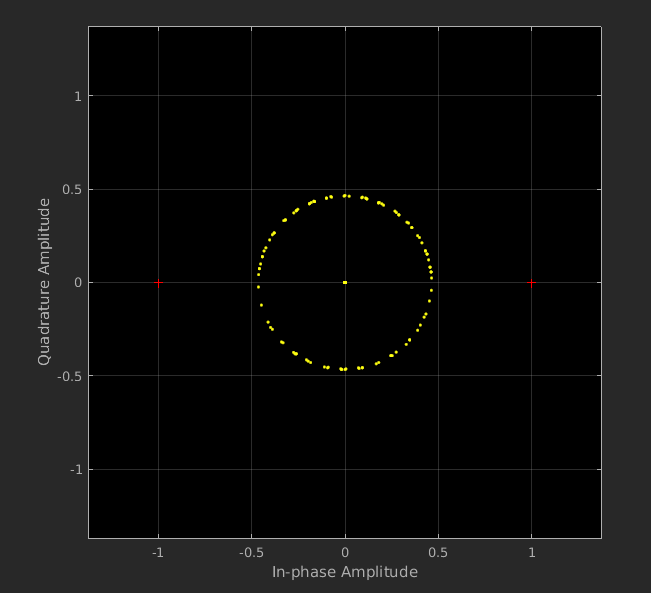
\includegraphics[width=8cm]{gfx/images/freqd-correlation}
	\caption{Cross Correlation of Frequency-Domain Symbols after Channel}
	\label{fig:freqd-corr}
\end{figure}

This kind of path effects is not at all unusual in a IEEE 802.11 transmission. Under normal circumstances, the known preamble is used to calculate the inverted channel matrix of the path effects, as mentioned in section \ref{sec:multipath}.

When receiving a collision, there is however not only one preamble. Instead, the preambles of two different frames, which experienced different path effects, are added together. Since the preambles themselves are designed to have a low off-peak autocorrelation \cite{ieee2012}, it is not easily possible to separate the two channel effects from each other. Therefore, I can not reverse the phase shift introduced on the \gls{OFDM} symbols containing the \gls{MAC} address.

As expected, experiments with cross-correlation in the frequency-domain without channel equalization were unsuccessful. I therefore disregarded this approach.


%% -----------------------------------------------------------------------------

\section{Time-Domain Correlation}

The experiments I did using time-domain cross-correlation are devided in two groups. First, I used Matlab to simulate different field variations and channel effects. Second, I used WARP boards to try the approach in a real-world scenario. The results of these experiments are summarized in the following sections.

When correlating time-domain samples, I always pre-generated reference samples and calculated the correlation only for the subset of samples that contains the \gls{MAC} address. Section \ref{sec:mac-periods} describes which period of the signal this is.\\

Reference signals are modulated until just after the \gls{IFFT} and adding of cyclic prefix. For the simulations, I used a sampling rate of 20 MHz, which is the default output of the Matlab WLAN System Toolbox. The WARP boards use a sampling frequency of 40 MHz however, so for these experiments I used interpolation to double the rate.

All experiments used realistic real-world \gls{MAC} addresses, as described in section \ref{sec:real-world-macs}.


%% -----------------------------------------------------------------------------

\section{Real-World MAC Addresses}\label{sec:real-world-macs}

\gls{MAC} addresses are 6 byte numbers, where the first 3 bytes are a vendor prefix, identifying the company that built the network interface. The remaining 3 bytes are a unique identifier for the specific hardware.

After initial tries with some artificial \gls{MAC} addresses in the form of \texttt{AB:CD:EF:12:34:56}, I switched to using a sample set of real-world \gls{MAC} addresses. This allowed for a closer simulation of an actual use-case for sender detection.\\

I collected 64 \gls{MAC} addresses from devices that were connected to the wireless university eduroam network. The gathering was done in the afternoon on a weekday. I used airodump from the \texttt{aircrack-ng} software suite to dump all \gls{MAC} addresses on the network into a file. The actual command looked like this:

\begin{lstlisting}[captionpos=b,caption={Capture Real-World MAC Addresses},label=lst:airodump]
airmon-ng start wlp0s20u1
airodump-ng --essid eduroam -a -o csv -w mac-addresses-eduroam.csv wlp0s20u1mon
\end{lstlisting}

It is important to have the wireless network interface set to promiscuous mode. This mode instructs the driver to hand all received frames to the kernel. Otherwise, only frames that are addressed to or coming from the local station are gathered, while the rest is filtered. This would mean that only the router's and the station's own \gls{MAC} address would be cached.

In a possible real-time usage scenario of the sender detection algorithm, it would also be important to use promiscuous mode in order to collect all \gls{MAC} addresses. These are the addresses for which reference signals need to be modulated and cached.


%% -----------------------------------------------------------------------------

\section{Modulation and Coding Schemes}

Intuitively, the overall sender detection accuracy should decrease for higher \glspl{MCS}. Firstly, with a higher \gls{MCS} there are more payload bits encoded in every \gls{OFDM} symbol, as described in table \ref{tbl:mcs}. This means that when applying cross-correlation, the \gls{OFDM} symbol contains random data from the \gls{MAC} header before and after the sender \gls{MAC} address. Due to the nature of \gls{OFDM}, it is not possible to limit correlation to only a fraction of the symbol in the time-domain.

Secondly, the higher constellation itself, which comes with higher \gls{MCS}, means that payload data gets mapped to complex points in the constellation plane that are less distinct from each other. Therefore, different data can be more similar under cross-correlation, making it harder to detect senders in the time-domain.\\

To evaluate the detection algorithm's performance, I measured the correctness of detected \gls{MAC} addresses for each of the 8 available \glspl{MCS}. For every \gls{MCS}, 1000 runs were performed. The results are the stacked sums of times where a completely correct pair of senders were guessed, times where only one of the senders was correct, and the amount of failures, in the sense of both addresses being incorrect.

Figure \ref{fig:vary_mcs} is the resulting plot. Different \glspl{MCS} are spread out on the x axis. The stacked bars show the amount of experiments for each result category as described above. As expected, the detection accuracy decreases for higher \glspl{MCS}. It is worth mentioning that for low \glspl{MCS}, the performance is very good, better than I expected. Furthermore, it seems to decrease exponentionally, but to justify this more data would be needed.

\begin{figure}[H]
	\centering
  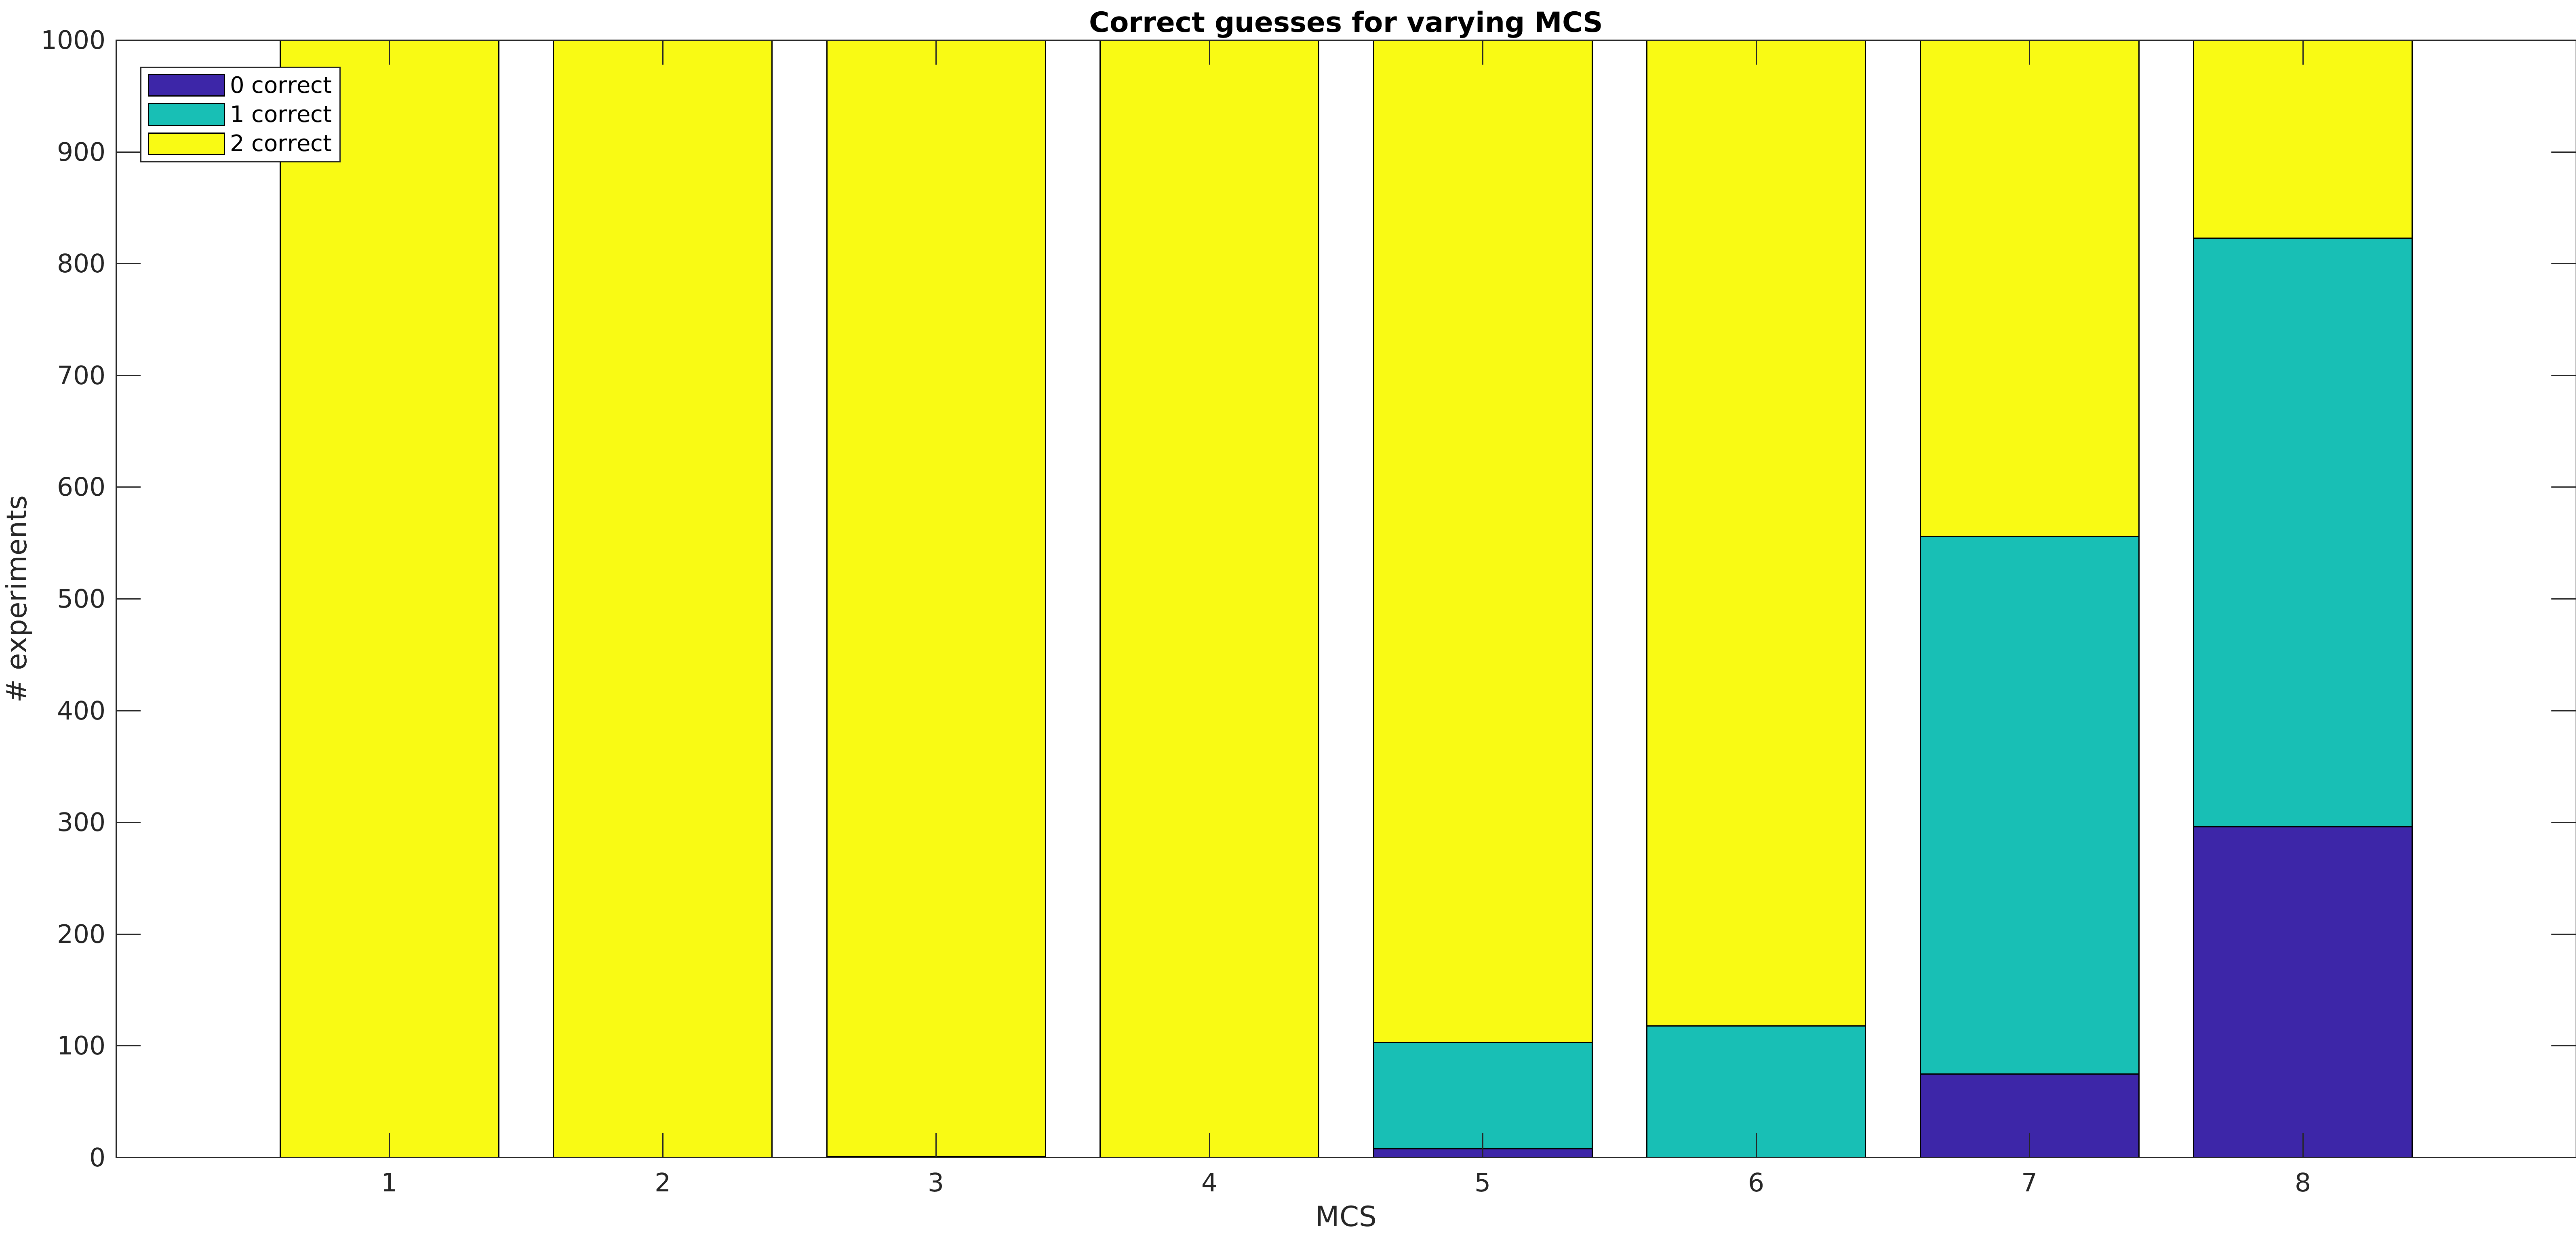
\includegraphics[width=\textwidth]{gfx/plots/vary_mcs-20170608-1859-num_correct-64_addresses-1000_experiments.png}
	\caption{Results: Varying MCS for 1000 Runs}
	\label{fig:vary_mcs}
\end{figure}


%% -----------------------------------------------------------------------------

\section{Scrambler Initialization}\label{sec:ex-scrambler}

As described in section \ref{sec:mac-and-phy}, the \gls{MAC} layer payload data is scrambled before any modulation on the physical layer is applied. The scrambling uses a 7 bit state register, where 0 is no valid state. Therefore, 127 unique scrambler initialization values are possible.

If the scrambler initialization is important for the sender detection technique, specifically if the modulated reference signals must use the same initialization as the received frames, the amount of possible values linearly scales the algorithm's complexity. That is, for every cached \gls{MAC} address, \gls{MCS} et cetera all scrambler initializations must be modulated and correlated. It is therefore very interesting to know whether that is the case, or whether the scrambler alternatively does not affect detection quality.\\

Figure \ref{fig:vary_scrambler} shows the detection performance for different scrambler initializations over 1000 experiments. The data is presented the same way as in the previous section as stacked bar plots denoting the amount of runs with 0, 1, and 2 corrects guesses. For all experiments, the \gls{MCS} 0 was used. While the simulated received frame was modulated with scrambler initialization 1, correlation was calculated against 127 reference signals with different scrambler values.

The results show that indeed the scrambler initialization is very important for detection quality. While the performance is very good for the correct initialization value 1, for all other values the accuracy is low. However, related research mentions that some network interfaces seem to not choose the scrambler initialization at random \cite{noubir2016}, contradictory to the IEEE 802.11 standard. These devices use a static initialization for every frame, or increment the value after every transmission. This could be exploited by limiting the reference signals to such that are expected in the current network, therefore avoiding time spent on correlations that are unpromising. Since the \gls{MAC} addresses of stations in the network are cached, the interface types and vendors are known. This could lead to some interesting future work.

\begin{figure}[H]
	\centering
	% uncomment the following line to recompile the figure when it changes otherwise a cached version is used
	%\tikzset{external/remake next}
	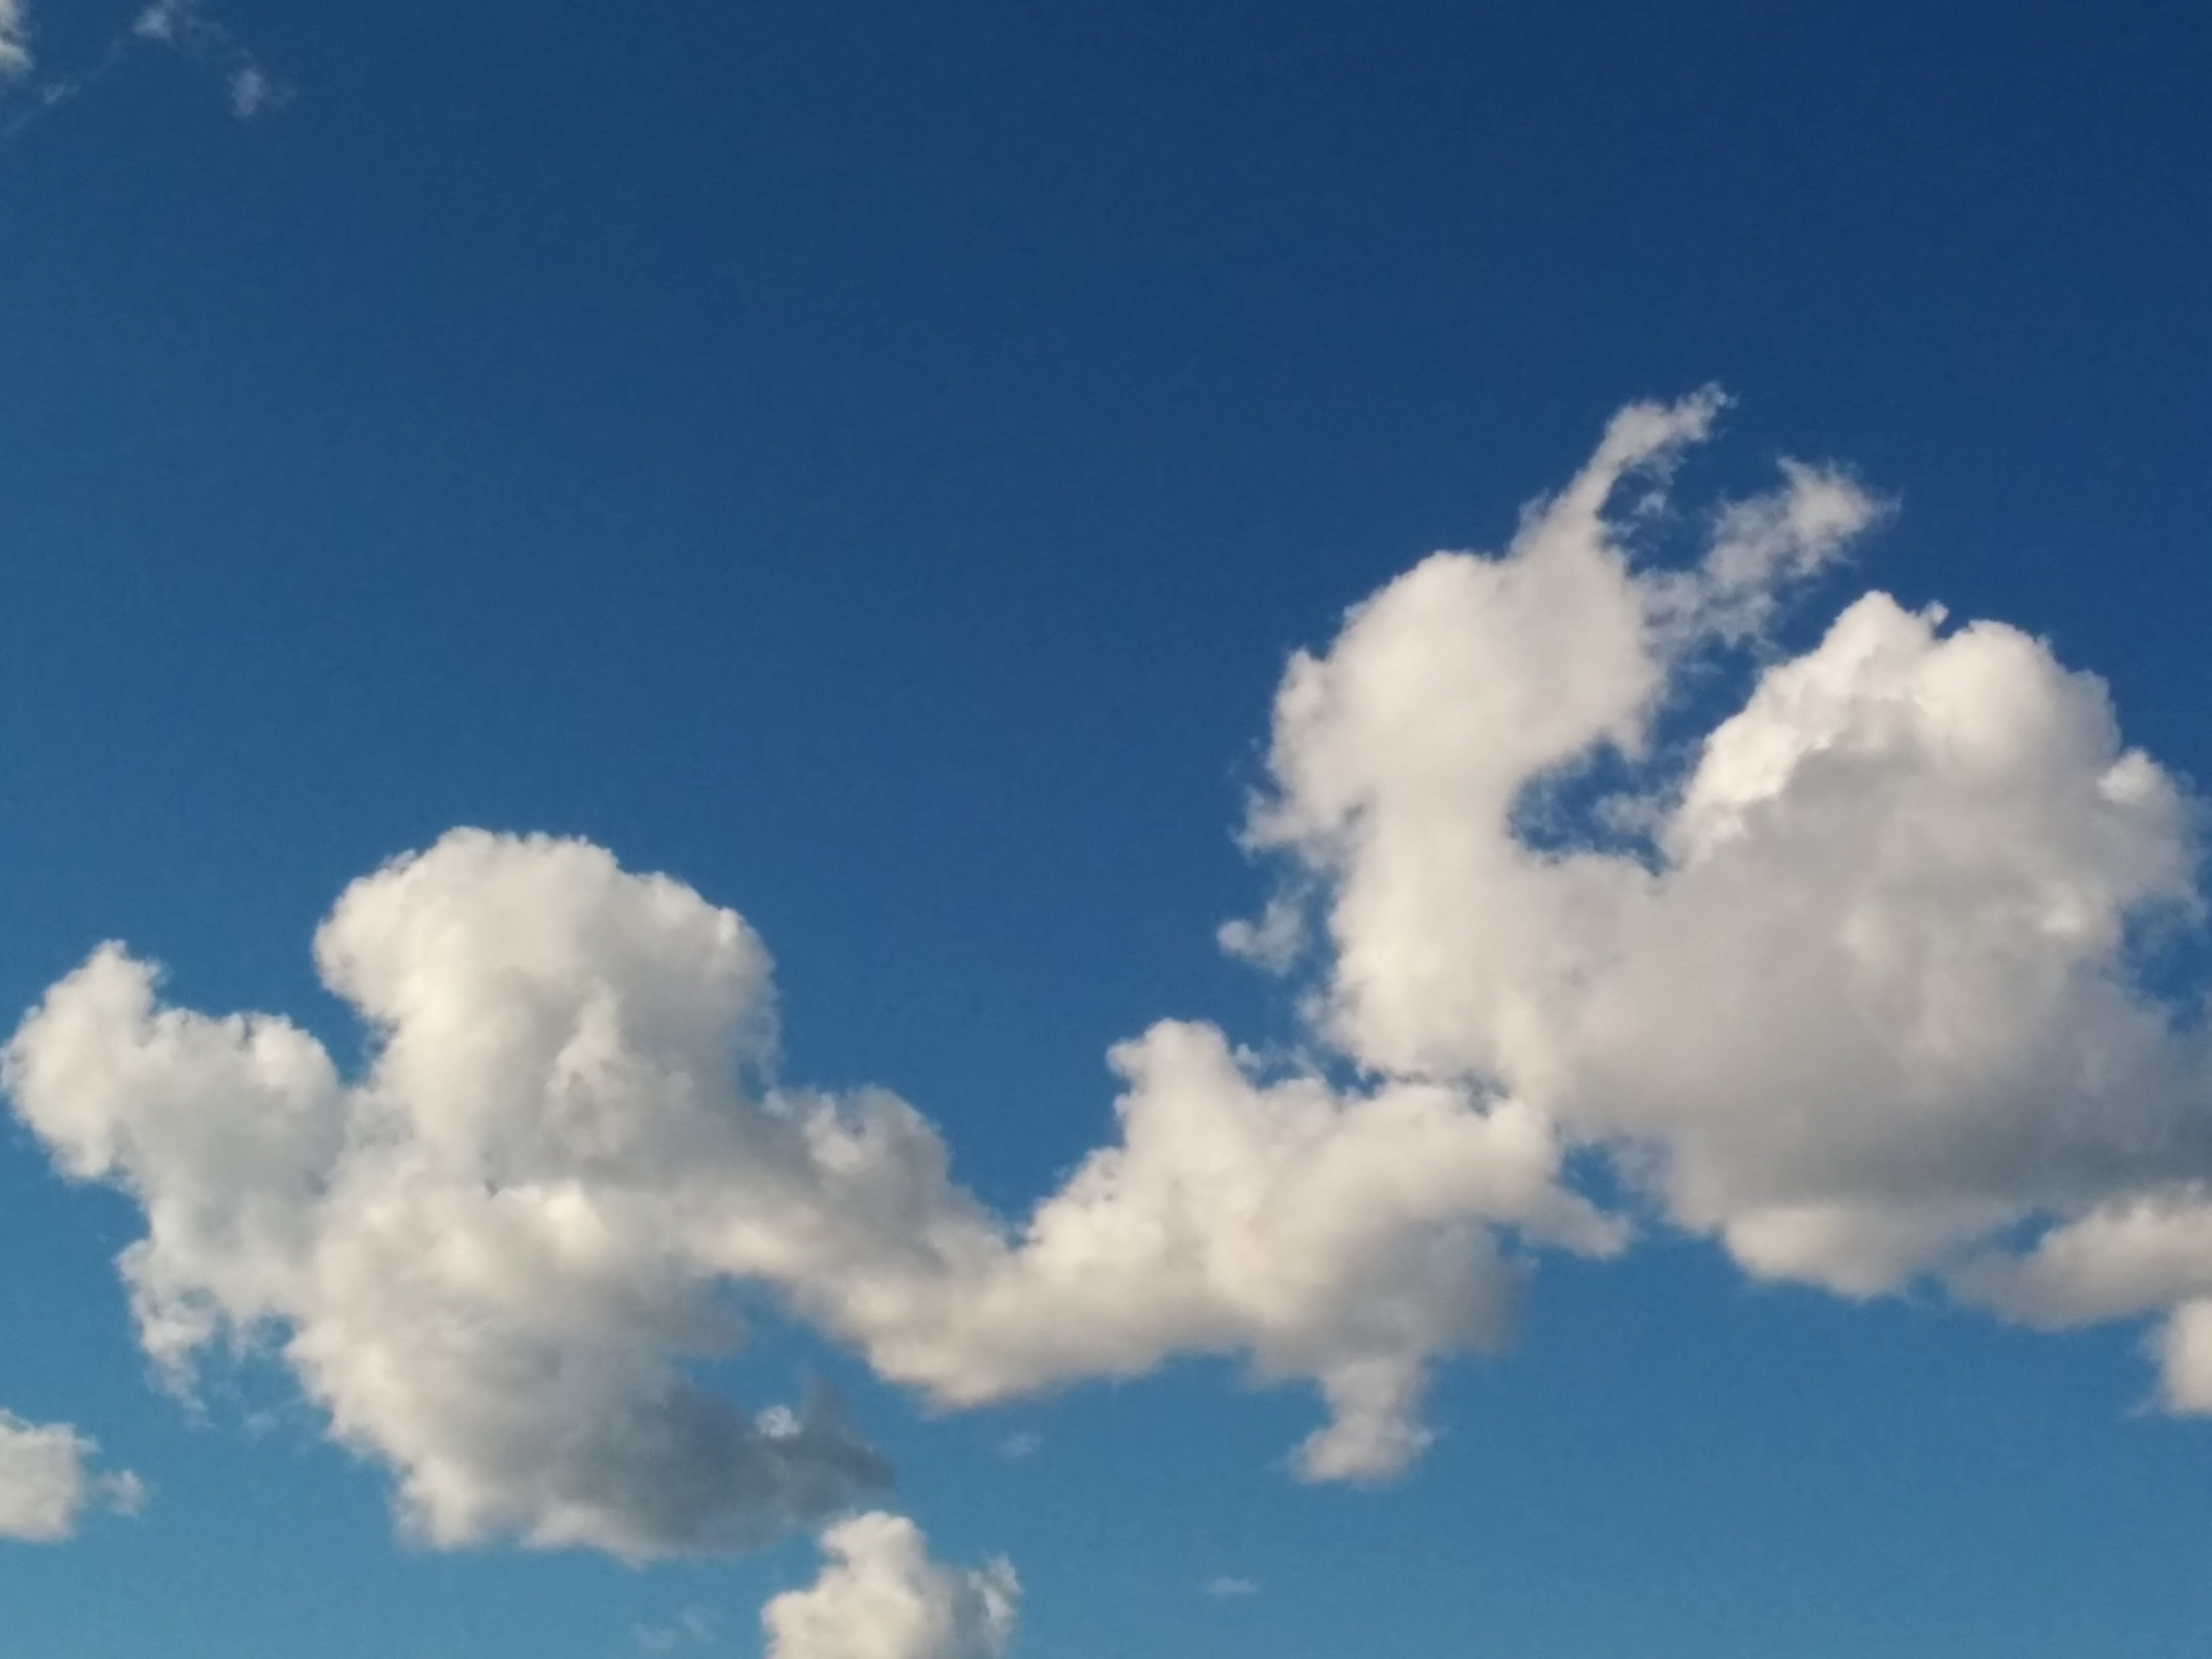
\includegraphics[width=0.9\textwidth,height=5cm]{gfx/images/stock-clouds}
	\caption[Results: Varying Scrambler Initialization for 1000 Experiments]{Results: Varying Scrambler Initialization for 1000 Runs at MCS 0}
	\label{fig:vary_scrambler}
\end{figure}


%% -----------------------------------------------------------------------------

\section{Preceding Data Variations}\label{sec:ex-destination}

Similar to the scrambler initialization, the \gls{MAC} header field preceding the sender \gls{MAC} address could also influence detection quality. This is due to the convolutional encoder as described in section \ref{sec:mac-and-phy}. The field before the sender \gls{MAC} address in a data frame is the destination \gls{MAC} address. In the following experiment, I measured to which extent the value of the destination address affects the accuracy of my detection technique.\\

Figure \ref{fig:vary_dest} shows the results in the same way as for the previous figures. Since the convolutional encoder uses a 7 bit state, only the last 7 bits of the destination \gls{MAC} address matter. After these last 7 bits, the register is synchronized to the same state, regardless of the preceding first 41 bits of the address. This makes up for a total of 128 different values that are evaluated with 1000 experiments each. As for the scrambler initialization, the experiments are done at \gls{MCS} 0.

\begin{figure}[H]
	\centering
	% uncomment the following line to recompile the figure when it changes otherwise a cached version is used
	%\tikzset{external/remake next}
	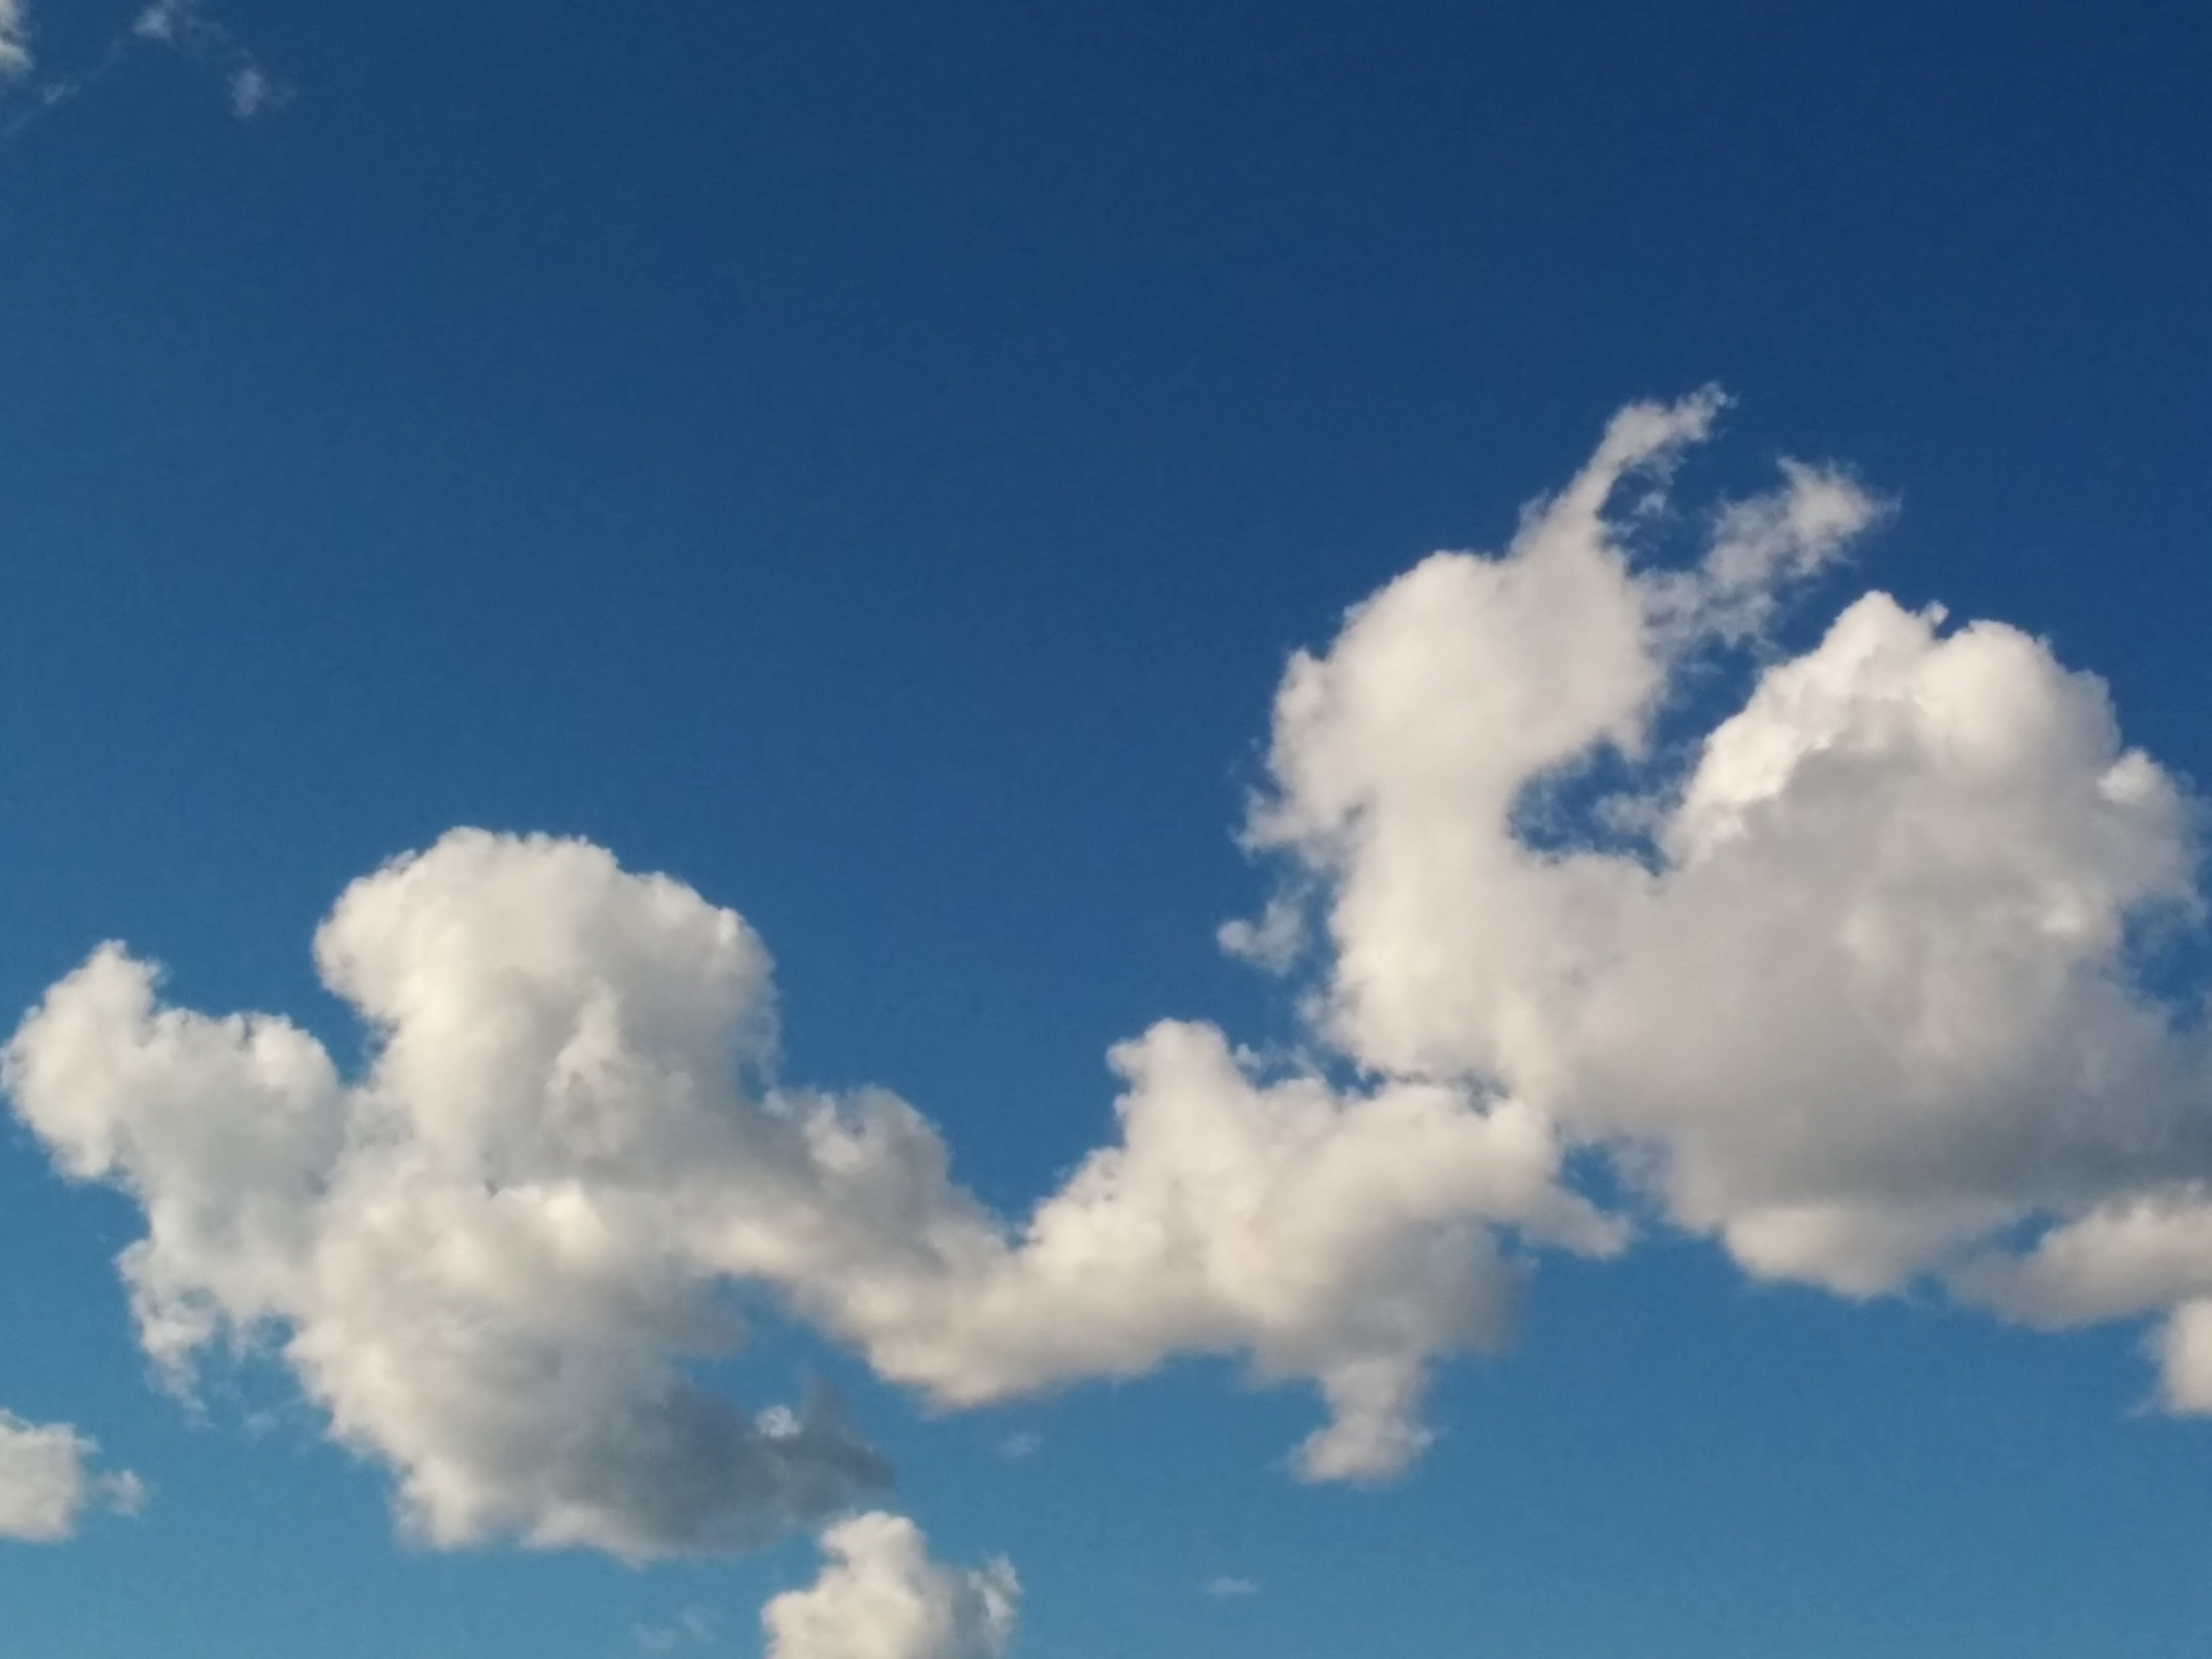
\includegraphics[width=0.9\textwidth,height=5cm]{gfx/images/stock-clouds}
	\caption[Results: Varying Destination \gls{MAC} Address for 1000 Experiments]{Results: Varying Destination \gls{MAC} Address for 1000 Experiments at MCS 0}
	\label{fig:vary_dest}
\end{figure}

It turns out that unlike the scrambler initialization, preceding payload data does not really have a measurable effect. Detection quality is comparable regardless of the trailing bits of the \gls{MAC} address. I discuss possible reasons for this in section \ref{sec:detection-quality}. An important implication of this result is that it is not necessary to check all 128 possible encoder states for every collision in real-time, which would be another linear scaling factor for the computational complexity of the algorithm.


%% -----------------------------------------------------------------------------

\section{Channel Models}

So far, all experiments were done in simulations with an ideal channel, meaning there were no path effects such as multi-path fading or attenuation. As this is not very realistic, I will evaluate performance under various channel models in this section.\\

Using Matlab, there are different models available that could be applied. On the one hand, the Communications System Toolbox comes with \texttt{stdchan}, which supports the \texttt{802.11g} and \texttt{802.11g} channel types. These are suited quite well for this scenario. The channel models requires some parameters, including the sampling frequency, Doppler spread, and \gls{RMS} delay spread $ t_{RMS} $. The delay spread was varied from 100 ns to 500 ns in steps of 50 ns. The usage of the stdchan filter is illustrated by listing \ref{lst:stdchan}:

\begin{lstlisting}[captionpos=b,caption={Matlab stdchan Channel Model},label=lst:stdchan]
tmrs = ...;
fs = 20e6; % Hz Sampling Frequency
fd = 10; % Hz Doppler spread
chan = stdchan(1/fs, fd, '802.11g', trms);
rx = filter(chan, tx);
\end{lstlisting}

The results of this experiment are shown in figure \ref{fig:vary_trms}. For every \texttt{trms} value, 1000 runs were performed. The process was repeated for all eight \glspl{MCS}.

On the other hand, the WLAN Systems Toolbox comes with a number of specifically drafted IEEE 802.11 channel models. These are designed according to the IEEE 802.11 standard models described in the specification \cite{ieee2012}. There are 6 models (A to F), of which I used the following three:

\begin{itemize}
	\item \textit{Model B}: typical large open space and office environments, no line-of-sight, 100 ns \gls{RMS} delay spread
	\item \textit{Model D}: large open space (indoor and outdoor), line-of-sight conditions, 140 ns \gls{RMS} delay spread
	\item \textit{Model E}: typical large open space (indoor and outdoor), no line-of-sight, 250 ns \gls{RMS} delay spread
\end{itemize}

I use the \texttt{wlanTGnChannel} class. Technically, this channel is designed to be used with IEEE 802.11 n high-throughput networks. However, the class supports configuration of \gls{MIMO} streams. I set those to 1 antenna for transmission and reception, respectively. This should provide appropriate conditions for \gls{SISO} 802.11 a/g networks.

The channel is used with Matlab code similar to listing \ref{lst:tgn}. As for the \texttt{stdchan} invocation, the sampling rate must be passed to the function. I use path-loss and shadowing for fading, and configure \gls{SISO}.

\begin{lstlisting}[captionpos=b,caption={Matlab wlanTGnChannel Simulation},label=lst:tgn]
model = ...; % 'Model-B', 'Model-D', etc.
tgnchan = wlanTGnChannel( ...
        'SampleRate', 20e6, ... % Hz
        'LargeScaleFadingEffect', 'Pathloss and shadowing', ...
        'NumTransmitAntennas', 1, 'NumReceiveAntennas', 1, ... % SISO
        'DelayProfile', model);
rx = tgnchan(tx);
\end{lstlisting}

The results of the experiments are shown in figure \ref{fig:vary_tgn}. For each of the three channel models, 1000 runs were performed at each \gls{MCS}.

\begin{figure}[p]
	\centering
	\setlength\figureheight{3cm}
	\setlength\figurewidth{0.40\textwidth}
	\begin{tabular}{cc}
		% uncomment the following line to recompile the figure when it changes otherwise a cached version is used
		%\tikzset{external/remake next}
		\subfloat[MCS 0]{% This file was created by matlab2tikz.
%
%The latest updates can be retrieved from
%  http://www.mathworks.com/matlabcentral/fileexchange/22022-matlab2tikz-matlab2tikz
%where you can also make suggestions and rate matlab2tikz.
%
\definecolor{mycolor1}{rgb}{0.24220,0.15040,0.66030}%
\definecolor{mycolor2}{rgb}{0.09640,0.75000,0.71204}%
\definecolor{mycolor3}{rgb}{0.97690,0.98390,0.08050}%
%
\begin{tikzpicture}[%
font=\footnotesize
]

\begin{axis}[%
width=0.951\figurewidth,
height=\figureheight,
at={(0\figurewidth,0\figureheight)},
scale only axis,
bar width=0,
xmin=5e-08,
xmax=5.5e-07,
xlabel style={font=\color{white!15!black}},
xlabel={$\text{802.11g stdchan: t}_\text{R}\text{MS in seconds}$},
ymin=0,
ymax=10,
ylabel style={font=\color{white!15!black}},
ylabel={\# experiments},
axis background/.style={fill=white},
title style={font=\bfseries},
title={MCS 0},
legend style={legend cell align=left, align=left, draw=white!15!black},
clip mode=individual,transpose legend,legend columns=2,legend style={at={(0,1)},anchor=north west,draw=black,fill=white,legend cell align=left}
]
\addplot[ybar stacked, fill=mycolor1, draw=black, area legend] table[row sep=crcr] {%
1e-07	0\\
1.5e-07	0\\
2e-07	0\\
2.5e-07	0\\
3e-07	0\\
3.5e-07	0\\
4e-07	0\\
4.5e-07	0\\
5e-07	0\\
};
\addplot[forget plot, color=white!15!black] table[row sep=crcr] {%
5e-08	0\\
5.5e-07	0\\
};
\addlegendentry{0 correct}

\addplot[ybar stacked, fill=mycolor2, draw=black, area legend] table[row sep=crcr] {%
1e-07	5\\
1.5e-07	3\\
2e-07	8\\
2.5e-07	4\\
3e-07	6\\
3.5e-07	7\\
4e-07	8\\
4.5e-07	7\\
5e-07	7\\
};
\addplot[forget plot, color=white!15!black] table[row sep=crcr] {%
5e-08	0\\
5.5e-07	0\\
};
\addlegendentry{1 correct}

\addplot[ybar stacked, fill=mycolor3, draw=black, area legend] table[row sep=crcr] {%
1e-07	5\\
1.5e-07	7\\
2e-07	2\\
2.5e-07	6\\
3e-07	4\\
3.5e-07	3\\
4e-07	2\\
4.5e-07	3\\
5e-07	3\\
};
\addplot[forget plot, color=white!15!black] table[row sep=crcr]  &
		\subfloat[MCS 1]{% This file was created by matlab2tikz.
%
%The latest updates can be retrieved from
%  http://www.mathworks.com/matlabcentral/fileexchange/22022-matlab2tikz-matlab2tikz
%where you can also make suggestions and rate matlab2tikz.
%
\definecolor{mycolor1}{rgb}{0.24220,0.15040,0.66030}%
\definecolor{mycolor2}{rgb}{0.09640,0.75000,0.71204}%
\definecolor{mycolor3}{rgb}{0.97690,0.98390,0.08050}%
%
\begin{tikzpicture}[%
font=\footnotesize
]

\begin{axis}[%
width=0.951\figurewidth,
height=\figureheight,
at={(0\figurewidth,0\figureheight)},
scale only axis,
bar width=0,
xmin=5e-08,
xmax=5.5e-07,
xlabel style={font=\color{white!15!black}},
xlabel={$\text{802.11g stdchan: t}_\text{R}\text{MS in seconds}$},
ymin=0,
ymax=10,
ylabel style={font=\color{white!15!black}},
ylabel={\# experiments},
axis background/.style={fill=white},
title style={font=\bfseries},
title={MCS 1},
legend style={legend cell align=left, align=left, draw=white!15!black},
clip mode=individual,transpose legend,legend columns=2,legend style={at={(0,1)},anchor=north west,draw=black,fill=white,legend cell align=left}
]
\addplot[ybar stacked, fill=mycolor1, draw=black, area legend] table[row sep=crcr] {%
1e-07	0\\
1.5e-07	0\\
2e-07	0\\
2.5e-07	1\\
3e-07	4\\
3.5e-07	2\\
4e-07	6\\
4.5e-07	5\\
5e-07	4\\
};
\addplot[forget plot, color=white!15!black] table[row sep=crcr] {%
5e-08	0\\
5.5e-07	0\\
};
\addlegendentry{0 correct}

\addplot[ybar stacked, fill=mycolor2, draw=black, area legend] table[row sep=crcr] {%
1e-07	6\\
1.5e-07	6\\
2e-07	10\\
2.5e-07	7\\
3e-07	5\\
3.5e-07	7\\
4e-07	3\\
4.5e-07	5\\
5e-07	5\\
};
\addplot[forget plot, color=white!15!black] table[row sep=crcr] {%
5e-08	0\\
5.5e-07	0\\
};
\addlegendentry{1 correct}

\addplot[ybar stacked, fill=mycolor3, draw=black, area legend] table[row sep=crcr] {%
1e-07	4\\
1.5e-07	4\\
2e-07	0\\
2.5e-07	2\\
3e-07	1\\
3.5e-07	1\\
4e-07	1\\
4.5e-07	0\\
5e-07	1\\
};
\addplot[forget plot, color=white!15!black] table[row sep=crcr]  \\
		\subfloat[MCS 2]{% This file was created by matlab2tikz.
%
%The latest updates can be retrieved from
%  http://www.mathworks.com/matlabcentral/fileexchange/22022-matlab2tikz-matlab2tikz
%where you can also make suggestions and rate matlab2tikz.
%
\definecolor{mycolor1}{rgb}{0.24220,0.15040,0.66030}%
\definecolor{mycolor2}{rgb}{0.09640,0.75000,0.71204}%
\definecolor{mycolor3}{rgb}{0.97690,0.98390,0.08050}%
%
\begin{tikzpicture}[%
font=\footnotesize
]

\begin{axis}[%
width=0.951\figurewidth,
height=\figureheight,
at={(0\figurewidth,0\figureheight)},
scale only axis,
bar width=0,
xmin=5e-08,
xmax=5.5e-07,
xlabel style={font=\color{white!15!black}},
xlabel={$\text{802.11g stdchan: t}_\text{R}\text{MS in seconds}$},
ymin=0,
ymax=10,
ylabel style={font=\color{white!15!black}},
ylabel={\# experiments},
axis background/.style={fill=white},
title style={font=\bfseries},
title={MCS 2},
legend style={legend cell align=left, align=left, draw=white!15!black},
clip mode=individual,transpose legend,legend columns=2,legend style={at={(0,1)},anchor=north west,draw=black,fill=white,legend cell align=left}
]
\addplot[ybar stacked, fill=mycolor1, draw=black, area legend] table[row sep=crcr] {%
1e-07	0\\
1.5e-07	0\\
2e-07	0\\
2.5e-07	0\\
3e-07	1\\
3.5e-07	4\\
4e-07	1\\
4.5e-07	3\\
5e-07	3\\
};
\addplot[forget plot, color=white!15!black] table[row sep=crcr] {%
5e-08	0\\
5.5e-07	0\\
};
\addlegendentry{0 correct}

\addplot[ybar stacked, fill=mycolor2, draw=black, area legend] table[row sep=crcr] {%
1e-07	7\\
1.5e-07	7\\
2e-07	9\\
2.5e-07	9\\
3e-07	7\\
3.5e-07	5\\
4e-07	7\\
4.5e-07	6\\
5e-07	7\\
};
\addplot[forget plot, color=white!15!black] table[row sep=crcr] {%
5e-08	0\\
5.5e-07	0\\
};
\addlegendentry{1 correct}

\addplot[ybar stacked, fill=mycolor3, draw=black, area legend] table[row sep=crcr] {%
1e-07	3\\
1.5e-07	3\\
2e-07	1\\
2.5e-07	1\\
3e-07	2\\
3.5e-07	1\\
4e-07	2\\
4.5e-07	1\\
5e-07	0\\
};
\addplot[forget plot, color=white!15!black] table[row sep=crcr]  &
		\subfloat[MCS 3]{% This file was created by matlab2tikz.
%
%The latest updates can be retrieved from
%  http://www.mathworks.com/matlabcentral/fileexchange/22022-matlab2tikz-matlab2tikz
%where you can also make suggestions and rate matlab2tikz.
%
\definecolor{mycolor1}{rgb}{0.24220,0.15040,0.66030}%
\definecolor{mycolor2}{rgb}{0.09640,0.75000,0.71204}%
\definecolor{mycolor3}{rgb}{0.97690,0.98390,0.08050}%
%
\begin{tikzpicture}[%
font=\footnotesize
]

\begin{axis}[%
width=0.951\figurewidth,
height=\figureheight,
at={(0\figurewidth,0\figureheight)},
scale only axis,
bar width=0,
xmin=5e-08,
xmax=5.5e-07,
xlabel style={font=\color{white!15!black}},
xlabel={$\text{802.11g stdchan: t}_\text{R}\text{MS in seconds}$},
ymin=0,
ymax=10,
ylabel style={font=\color{white!15!black}},
ylabel={\# experiments},
axis background/.style={fill=white},
title style={font=\bfseries},
title={MCS 3},
legend style={legend cell align=left, align=left, draw=white!15!black},
clip mode=individual,transpose legend,legend columns=2,legend style={at={(0,1)},anchor=north west,draw=black,fill=white,legend cell align=left}
]
\addplot[ybar stacked, fill=mycolor1, draw=black, area legend] table[row sep=crcr] {%
1e-07	1\\
1.5e-07	6\\
2e-07	2\\
2.5e-07	4\\
3e-07	4\\
3.5e-07	6\\
4e-07	6\\
4.5e-07	6\\
5e-07	6\\
};
\addplot[forget plot, color=white!15!black] table[row sep=crcr] {%
5e-08	0\\
5.5e-07	0\\
};
\addlegendentry{0 correct}

\addplot[ybar stacked, fill=mycolor2, draw=black, area legend] table[row sep=crcr] {%
1e-07	7\\
1.5e-07	2\\
2e-07	6\\
2.5e-07	6\\
3e-07	6\\
3.5e-07	4\\
4e-07	4\\
4.5e-07	4\\
5e-07	4\\
};
\addplot[forget plot, color=white!15!black] table[row sep=crcr] {%
5e-08	0\\
5.5e-07	0\\
};
\addlegendentry{1 correct}

\addplot[ybar stacked, fill=mycolor3, draw=black, area legend] table[row sep=crcr] {%
1e-07	2\\
1.5e-07	2\\
2e-07	2\\
2.5e-07	0\\
3e-07	0\\
3.5e-07	0\\
4e-07	0\\
4.5e-07	0\\
5e-07	0\\
};
\addplot[forget plot, color=white!15!black] table[row sep=crcr]  \\
		\subfloat[MCS 4]{% This file was created by matlab2tikz.
%
%The latest updates can be retrieved from
%  http://www.mathworks.com/matlabcentral/fileexchange/22022-matlab2tikz-matlab2tikz
%where you can also make suggestions and rate matlab2tikz.
%
\definecolor{mycolor1}{rgb}{0.24220,0.15040,0.66030}%
\definecolor{mycolor2}{rgb}{0.09640,0.75000,0.71204}%
\definecolor{mycolor3}{rgb}{0.97690,0.98390,0.08050}%
%
\begin{tikzpicture}[%
font=\footnotesize
]

\begin{axis}[%
width=0.951\figurewidth,
height=\figureheight,
at={(0\figurewidth,0\figureheight)},
scale only axis,
bar width=0,
xmin=5e-08,
xmax=5.5e-07,
xlabel style={font=\color{white!15!black}},
xlabel={$\text{802.11g stdchan: t}_\text{R}\text{MS in seconds}$},
ymin=0,
ymax=10,
ylabel style={font=\color{white!15!black}},
ylabel={\# experiments},
axis background/.style={fill=white},
title style={font=\bfseries},
title={MCS 4},
legend style={legend cell align=left, align=left, draw=white!15!black},
clip mode=individual,transpose legend,legend columns=2,legend style={at={(0,1)},anchor=north west,draw=black,fill=white,legend cell align=left}
]
\addplot[ybar stacked, fill=mycolor1, draw=black, area legend] table[row sep=crcr] {%
1e-07	4\\
1.5e-07	6\\
2e-07	4\\
2.5e-07	4\\
3e-07	7\\
3.5e-07	7\\
4e-07	7\\
4.5e-07	7\\
5e-07	8\\
};
\addplot[forget plot, color=white!15!black] table[row sep=crcr] {%
5e-08	0\\
5.5e-07	0\\
};
\addlegendentry{0 correct}

\addplot[ybar stacked, fill=mycolor2, draw=black, area legend] table[row sep=crcr] {%
1e-07	4\\
1.5e-07	4\\
2e-07	6\\
2.5e-07	5\\
3e-07	3\\
3.5e-07	2\\
4e-07	3\\
4.5e-07	3\\
5e-07	2\\
};
\addplot[forget plot, color=white!15!black] table[row sep=crcr] {%
5e-08	0\\
5.5e-07	0\\
};
\addlegendentry{1 correct}

\addplot[ybar stacked, fill=mycolor3, draw=black, area legend] table[row sep=crcr] {%
1e-07	2\\
1.5e-07	0\\
2e-07	0\\
2.5e-07	1\\
3e-07	0\\
3.5e-07	1\\
4e-07	0\\
4.5e-07	0\\
5e-07	0\\
};
\addplot[forget plot, color=white!15!black] table[row sep=crcr]  &
		\subfloat[MCS 5]{% This file was created by matlab2tikz.
%
%The latest updates can be retrieved from
%  http://www.mathworks.com/matlabcentral/fileexchange/22022-matlab2tikz-matlab2tikz
%where you can also make suggestions and rate matlab2tikz.
%
\definecolor{mycolor1}{rgb}{0.24220,0.15040,0.66030}%
\definecolor{mycolor2}{rgb}{0.09640,0.75000,0.71204}%
\definecolor{mycolor3}{rgb}{0.97690,0.98390,0.08050}%
%
\begin{tikzpicture}[%
font=\footnotesize
]

\begin{axis}[%
width=0.951\figurewidth,
height=\figureheight,
at={(0\figurewidth,0\figureheight)},
scale only axis,
bar width=0,
xmin=5e-08,
xmax=5.5e-07,
xlabel style={font=\color{white!15!black}},
xlabel={$\text{802.11g stdchan: t}_\text{R}\text{MS in seconds}$},
ymin=0,
ymax=10,
ylabel style={font=\color{white!15!black}},
ylabel={\# experiments},
axis background/.style={fill=white},
title style={font=\bfseries},
title={MCS 5},
legend style={legend cell align=left, align=left, draw=white!15!black},
clip mode=individual,transpose legend,legend columns=2,legend style={at={(0,1)},anchor=north west,draw=black,fill=white,legend cell align=left}
]
\addplot[ybar stacked, fill=mycolor1, draw=black, area legend] table[row sep=crcr] {%
1e-07	0\\
1.5e-07	4\\
2e-07	3\\
2.5e-07	3\\
3e-07	4\\
3.5e-07	9\\
4e-07	4\\
4.5e-07	7\\
5e-07	8\\
};
\addplot[forget plot, color=white!15!black] table[row sep=crcr] {%
5e-08	0\\
5.5e-07	0\\
};
\addlegendentry{0 correct}

\addplot[ybar stacked, fill=mycolor2, draw=black, area legend] table[row sep=crcr] {%
1e-07	8\\
1.5e-07	6\\
2e-07	5\\
2.5e-07	6\\
3e-07	5\\
3.5e-07	1\\
4e-07	6\\
4.5e-07	3\\
5e-07	2\\
};
\addplot[forget plot, color=white!15!black] table[row sep=crcr] {%
5e-08	0\\
5.5e-07	0\\
};
\addlegendentry{1 correct}

\addplot[ybar stacked, fill=mycolor3, draw=black, area legend] table[row sep=crcr] {%
1e-07	2\\
1.5e-07	0\\
2e-07	2\\
2.5e-07	1\\
3e-07	1\\
3.5e-07	0\\
4e-07	0\\
4.5e-07	0\\
5e-07	0\\
};
\addplot[forget plot, color=white!15!black] table[row sep=crcr]  \\
		\subfloat[MCS 6]{% This file was created by matlab2tikz.
%
%The latest updates can be retrieved from
%  http://www.mathworks.com/matlabcentral/fileexchange/22022-matlab2tikz-matlab2tikz
%where you can also make suggestions and rate matlab2tikz.
%
\definecolor{mycolor1}{rgb}{0.24220,0.15040,0.66030}%
\definecolor{mycolor2}{rgb}{0.09640,0.75000,0.71204}%
\definecolor{mycolor3}{rgb}{0.97690,0.98390,0.08050}%
%
\begin{tikzpicture}[%
font=\footnotesize
]

\begin{axis}[%
width=0.951\figurewidth,
height=\figureheight,
at={(0\figurewidth,0\figureheight)},
scale only axis,
bar width=0,
xmin=5e-08,
xmax=5.5e-07,
xlabel style={font=\color{white!15!black}},
xlabel={$\text{802.11g stdchan: t}_\text{R}\text{MS in seconds}$},
ymin=0,
ymax=10,
ylabel style={font=\color{white!15!black}},
ylabel={\# experiments},
axis background/.style={fill=white},
title style={font=\bfseries},
title={MCS 6},
legend style={legend cell align=left, align=left, draw=white!15!black},
clip mode=individual,transpose legend,legend columns=2,legend style={at={(0,1)},anchor=north west,draw=black,fill=white,legend cell align=left}
]
\addplot[ybar stacked, fill=mycolor1, draw=black, area legend] table[row sep=crcr] {%
1e-07	5\\
1.5e-07	8\\
2e-07	6\\
2.5e-07	8\\
3e-07	7\\
3.5e-07	7\\
4e-07	8\\
4.5e-07	8\\
5e-07	6\\
};
\addplot[forget plot, color=white!15!black] table[row sep=crcr] {%
5e-08	0\\
5.5e-07	0\\
};
\addlegendentry{0 correct}

\addplot[ybar stacked, fill=mycolor2, draw=black, area legend] table[row sep=crcr] {%
1e-07	4\\
1.5e-07	2\\
2e-07	4\\
2.5e-07	2\\
3e-07	3\\
3.5e-07	3\\
4e-07	2\\
4.5e-07	2\\
5e-07	4\\
};
\addplot[forget plot, color=white!15!black] table[row sep=crcr] {%
5e-08	0\\
5.5e-07	0\\
};
\addlegendentry{1 correct}

\addplot[ybar stacked, fill=mycolor3, draw=black, area legend] table[row sep=crcr] {%
1e-07	1\\
1.5e-07	0\\
2e-07	0\\
2.5e-07	0\\
3e-07	0\\
3.5e-07	0\\
4e-07	0\\
4.5e-07	0\\
5e-07	0\\
};
\addplot[forget plot, color=white!15!black] table[row sep=crcr]  &
		\subfloat[MCS 7]{% This file was created by matlab2tikz.
%
%The latest updates can be retrieved from
%  http://www.mathworks.com/matlabcentral/fileexchange/22022-matlab2tikz-matlab2tikz
%where you can also make suggestions and rate matlab2tikz.
%
\definecolor{mycolor1}{rgb}{0.24220,0.15040,0.66030}%
\definecolor{mycolor2}{rgb}{0.09640,0.75000,0.71204}%
\definecolor{mycolor3}{rgb}{0.97690,0.98390,0.08050}%
%
\begin{tikzpicture}[%
font=\footnotesize
]

\begin{axis}[%
width=0.951\figurewidth,
height=\figureheight,
at={(0\figurewidth,0\figureheight)},
scale only axis,
bar width=0,
xmin=5e-08,
xmax=5.5e-07,
xlabel style={font=\color{white!15!black}},
xlabel={$\text{802.11g stdchan: t}_\text{R}\text{MS in seconds}$},
ymin=0,
ymax=10,
ylabel style={font=\color{white!15!black}},
ylabel={\# experiments},
axis background/.style={fill=white},
title style={font=\bfseries},
title={MCS 7},
legend style={legend cell align=left, align=left, draw=white!15!black},
clip mode=individual,transpose legend,legend columns=2,legend style={at={(0,1)},anchor=north west,draw=black,fill=white,legend cell align=left}
]
\addplot[ybar stacked, fill=mycolor1, draw=black, area legend] table[row sep=crcr] {%
1e-07	8\\
1.5e-07	7\\
2e-07	7\\
2.5e-07	8\\
3e-07	9\\
3.5e-07	10\\
4e-07	10\\
4.5e-07	8\\
5e-07	10\\
};
\addplot[forget plot, color=white!15!black] table[row sep=crcr] {%
5e-08	0\\
5.5e-07	0\\
};
\addlegendentry{0 correct}

\addplot[ybar stacked, fill=mycolor2, draw=black, area legend] table[row sep=crcr] {%
1e-07	2\\
1.5e-07	3\\
2e-07	3\\
2.5e-07	2\\
3e-07	1\\
3.5e-07	0\\
4e-07	0\\
4.5e-07	2\\
5e-07	0\\
};
\addplot[forget plot, color=white!15!black] table[row sep=crcr] {%
5e-08	0\\
5.5e-07	0\\
};
\addlegendentry{1 correct}

\addplot[ybar stacked, fill=mycolor3, draw=black, area legend] table[row sep=crcr] {%
1e-07	0\\
1.5e-07	0\\
2e-07	0\\
2.5e-07	0\\
3e-07	0\\
3.5e-07	0\\
4e-07	0\\
4.5e-07	0\\
5e-07	0\\
};
\addplot[forget plot, color=white!15!black] table[row sep=crcr]  \\
	\end{tabular}
	\caption{Results: Varying $t_{RMS}$ in a Standard Channel for 1000 Runs}
	\label{fig:vary_trms}
\end{figure}

\begin{figure}[p]
	\centering
	\setlength\figureheight{3cm}
	\setlength\figurewidth{0.40\textwidth}
	\begin{tabular}{cc}
		% uncomment the following line to recompile the figure when it changes otherwise a cached version is used
		%\tikzset{external/remake next}
		\subfloat[MCS 0]{% This file was created by matlab2tikz.
%
%The latest updates can be retrieved from
%  http://www.mathworks.com/matlabcentral/fileexchange/22022-matlab2tikz-matlab2tikz
%where you can also make suggestions and rate matlab2tikz.
%
\definecolor{mycolor1}{rgb}{0.24220,0.15040,0.66030}%
\definecolor{mycolor2}{rgb}{0.09640,0.75000,0.71204}%
\definecolor{mycolor3}{rgb}{0.97690,0.98390,0.08050}%
%
\begin{tikzpicture}[%
font=\footnotesize
]

\begin{axis}[%
width=0.951\figurewidth,
height=\figureheight,
at={(0\figurewidth,0\figureheight)},
scale only axis,
bar width=0.8,
xmin=0.5,
xmax=3.5,
xtick={1,2,3},
xticklabels={{Model-B},{Model-D},{Model-E}},
xlabel style={font=\color{white!15!black}},
xlabel={AGWN SNR},
ymin=0,
ymax=100,
ylabel style={font=\color{white!15!black}},
ylabel={\# experiments},
axis background/.style={fill=white},
title style={font=\bfseries},
title={MCS 0},
legend style={legend cell align=left, align=left, draw=white!15!black},
clip mode=individual,transpose legend,legend columns=2,legend style={at={(0,1)},anchor=north west,draw=black,fill=white,legend cell align=left}
]
\addplot[ybar stacked, fill=mycolor1, draw=black, area legend] table[row sep=crcr] {%
1	0\\
2	0\\
3	0\\
};
\addplot[forget plot, color=white!15!black] table[row sep=crcr] {%
0.5	0\\
3.5	0\\
};
\addlegendentry{0 correct}

\addplot[ybar stacked, fill=mycolor2, draw=black, area legend] table[row sep=crcr] {%
1	0\\
2	0\\
3	1\\
};
\addplot[forget plot, color=white!15!black] table[row sep=crcr] {%
0.5	0\\
3.5	0\\
};
\addlegendentry{1 correct}

\addplot[ybar stacked, fill=mycolor3, draw=black, area legend] table[row sep=crcr] {%
1	100\\
2	100\\
3	99\\
};
\addplot[forget plot, color=white!15!black] table[row sep=crcr]  &
		\subfloat[MCS 1]{% This file was created by matlab2tikz.
%
%The latest updates can be retrieved from
%  http://www.mathworks.com/matlabcentral/fileexchange/22022-matlab2tikz-matlab2tikz
%where you can also make suggestions and rate matlab2tikz.
%
\definecolor{mycolor1}{rgb}{0.24220,0.15040,0.66030}%
\definecolor{mycolor2}{rgb}{0.09640,0.75000,0.71204}%
\definecolor{mycolor3}{rgb}{0.97690,0.98390,0.08050}%
%
\begin{tikzpicture}[%
font=\footnotesize
]

\begin{axis}[%
width=0.951\figurewidth,
height=\figureheight,
at={(0\figurewidth,0\figureheight)},
scale only axis,
bar width=0.8,
xmin=0.5,
xmax=3.5,
xtick={1,2,3},
xticklabels={{Model-B},{Model-D},{Model-E}},
xlabel style={font=\color{white!15!black}},
xlabel={AGWN SNR},
ymin=0,
ymax=100,
ylabel style={font=\color{white!15!black}},
ylabel={\# experiments},
axis background/.style={fill=white},
title style={font=\bfseries},
title={MCS 1},
legend style={legend cell align=left, align=left, draw=white!15!black},
clip mode=individual,transpose legend,legend columns=2,legend style={at={(0,1)},anchor=north west,draw=black,fill=white,legend cell align=left}
]
\addplot[ybar stacked, fill=mycolor1, draw=black, area legend] table[row sep=crcr] {%
1	5\\
2	7\\
3	13\\
};
\addplot[forget plot, color=white!15!black] table[row sep=crcr] {%
0.5	0\\
3.5	0\\
};
\addlegendentry{0 correct}

\addplot[ybar stacked, fill=mycolor2, draw=black, area legend] table[row sep=crcr] {%
1	1\\
2	2\\
3	3\\
};
\addplot[forget plot, color=white!15!black] table[row sep=crcr] {%
0.5	0\\
3.5	0\\
};
\addlegendentry{1 correct}

\addplot[ybar stacked, fill=mycolor3, draw=black, area legend] table[row sep=crcr] {%
1	94\\
2	91\\
3	84\\
};
\addplot[forget plot, color=white!15!black] table[row sep=crcr]  \\
		\subfloat[MCS 2]{% This file was created by matlab2tikz.
%
%The latest updates can be retrieved from
%  http://www.mathworks.com/matlabcentral/fileexchange/22022-matlab2tikz-matlab2tikz
%where you can also make suggestions and rate matlab2tikz.
%
\definecolor{mycolor1}{rgb}{0.24220,0.15040,0.66030}%
\definecolor{mycolor2}{rgb}{0.09640,0.75000,0.71204}%
\definecolor{mycolor3}{rgb}{0.97690,0.98390,0.08050}%
%
\begin{tikzpicture}[%
font=\footnotesize
]

\begin{axis}[%
width=0.951\figurewidth,
height=\figureheight,
at={(0\figurewidth,0\figureheight)},
scale only axis,
bar width=0.8,
xmin=0.5,
xmax=3.5,
xtick={1,2,3},
xticklabels={{Model-B},{Model-D},{Model-E}},
xlabel style={font=\color{white!15!black}},
xlabel={AGWN SNR},
ymin=0,
ymax=100,
ylabel style={font=\color{white!15!black}},
ylabel={\# experiments},
axis background/.style={fill=white},
title style={font=\bfseries},
title={MCS 2},
legend style={legend cell align=left, align=left, draw=white!15!black},
clip mode=individual,transpose legend,legend columns=2,legend style={at={(0,1)},anchor=north west,draw=black,fill=white,legend cell align=left}
]
\addplot[ybar stacked, fill=mycolor1, draw=black, area legend] table[row sep=crcr] {%
1	0\\
2	3\\
3	3\\
};
\addplot[forget plot, color=white!15!black] table[row sep=crcr] {%
0.5	0\\
3.5	0\\
};
\addlegendentry{0 correct}

\addplot[ybar stacked, fill=mycolor2, draw=black, area legend] table[row sep=crcr] {%
1	1\\
2	5\\
3	9\\
};
\addplot[forget plot, color=white!15!black] table[row sep=crcr] {%
0.5	0\\
3.5	0\\
};
\addlegendentry{1 correct}

\addplot[ybar stacked, fill=mycolor3, draw=black, area legend] table[row sep=crcr] {%
1	99\\
2	92\\
3	88\\
};
\addplot[forget plot, color=white!15!black] table[row sep=crcr]  &
		\subfloat[MCS 3]{% This file was created by matlab2tikz.
%
%The latest updates can be retrieved from
%  http://www.mathworks.com/matlabcentral/fileexchange/22022-matlab2tikz-matlab2tikz
%where you can also make suggestions and rate matlab2tikz.
%
\definecolor{mycolor1}{rgb}{0.24220,0.15040,0.66030}%
\definecolor{mycolor2}{rgb}{0.09640,0.75000,0.71204}%
\definecolor{mycolor3}{rgb}{0.97690,0.98390,0.08050}%
%
\begin{tikzpicture}[%
font=\footnotesize
]

\begin{axis}[%
width=0.951\figurewidth,
height=\figureheight,
at={(0\figurewidth,0\figureheight)},
scale only axis,
bar width=0.8,
xmin=0.5,
xmax=3.5,
xtick={1,2,3},
xticklabels={{Model-B},{Model-D},{Model-E}},
xlabel style={font=\color{white!15!black}},
xlabel={AGWN SNR},
ymin=0,
ymax=100,
ylabel style={font=\color{white!15!black}},
ylabel={\# experiments},
axis background/.style={fill=white},
title style={font=\bfseries},
title={MCS 3},
legend style={legend cell align=left, align=left, draw=white!15!black},
clip mode=individual,transpose legend,legend columns=2,legend style={at={(0,1)},anchor=north west,draw=black,fill=white,legend cell align=left}
]
\addplot[ybar stacked, fill=mycolor1, draw=black, area legend] table[row sep=crcr] {%
1	18\\
2	30\\
3	38\\
};
\addplot[forget plot, color=white!15!black] table[row sep=crcr] {%
0.5	0\\
3.5	0\\
};
\addlegendentry{0 correct}

\addplot[ybar stacked, fill=mycolor2, draw=black, area legend] table[row sep=crcr] {%
1	11\\
2	10\\
3	15\\
};
\addplot[forget plot, color=white!15!black] table[row sep=crcr] {%
0.5	0\\
3.5	0\\
};
\addlegendentry{1 correct}

\addplot[ybar stacked, fill=mycolor3, draw=black, area legend] table[row sep=crcr] {%
1	71\\
2	60\\
3	47\\
};
\addplot[forget plot, color=white!15!black] table[row sep=crcr]  \\
		\subfloat[MCS 4]{% This file was created by matlab2tikz.
%
%The latest updates can be retrieved from
%  http://www.mathworks.com/matlabcentral/fileexchange/22022-matlab2tikz-matlab2tikz
%where you can also make suggestions and rate matlab2tikz.
%
\definecolor{mycolor1}{rgb}{0.24220,0.15040,0.66030}%
\definecolor{mycolor2}{rgb}{0.09640,0.75000,0.71204}%
\definecolor{mycolor3}{rgb}{0.97690,0.98390,0.08050}%
%
\begin{tikzpicture}[%
font=\footnotesize
]

\begin{axis}[%
width=0.951\figurewidth,
height=\figureheight,
at={(0\figurewidth,0\figureheight)},
scale only axis,
bar width=0.8,
xmin=0.5,
xmax=3.5,
xtick={1,2,3},
xticklabels={{Model-B},{Model-D},{Model-E}},
xlabel style={font=\color{white!15!black}},
xlabel={AGWN SNR},
ymin=0,
ymax=100,
ylabel style={font=\color{white!15!black}},
ylabel={\# experiments},
axis background/.style={fill=white},
title style={font=\bfseries},
title={MCS 4},
legend style={legend cell align=left, align=left, draw=white!15!black},
clip mode=individual,transpose legend,legend columns=2,legend style={at={(0,1)},anchor=north west,draw=black,fill=white,legend cell align=left}
]
\addplot[ybar stacked, fill=mycolor1, draw=black, area legend] table[row sep=crcr] {%
1	9\\
2	36\\
3	47\\
};
\addplot[forget plot, color=white!15!black] table[row sep=crcr] {%
0.5	0\\
3.5	0\\
};
\addlegendentry{0 correct}

\addplot[ybar stacked, fill=mycolor2, draw=black, area legend] table[row sep=crcr] {%
1	29\\
2	30\\
3	26\\
};
\addplot[forget plot, color=white!15!black] table[row sep=crcr] {%
0.5	0\\
3.5	0\\
};
\addlegendentry{1 correct}

\addplot[ybar stacked, fill=mycolor3, draw=black, area legend] table[row sep=crcr] {%
1	62\\
2	34\\
3	27\\
};
\addplot[forget plot, color=white!15!black] table[row sep=crcr]  &
		\subfloat[MCS 5]{% This file was created by matlab2tikz.
%
%The latest updates can be retrieved from
%  http://www.mathworks.com/matlabcentral/fileexchange/22022-matlab2tikz-matlab2tikz
%where you can also make suggestions and rate matlab2tikz.
%
\definecolor{mycolor1}{rgb}{0.24220,0.15040,0.66030}%
\definecolor{mycolor2}{rgb}{0.09640,0.75000,0.71204}%
\definecolor{mycolor3}{rgb}{0.97690,0.98390,0.08050}%
%
\begin{tikzpicture}[%
font=\footnotesize
]

\begin{axis}[%
width=0.951\figurewidth,
height=\figureheight,
at={(0\figurewidth,0\figureheight)},
scale only axis,
bar width=0.8,
xmin=0.5,
xmax=3.5,
xtick={1,2,3},
xticklabels={{Model-B},{Model-D},{Model-E}},
xlabel style={font=\color{white!15!black}},
xlabel={AGWN SNR},
ymin=0,
ymax=100,
ylabel style={font=\color{white!15!black}},
ylabel={\# experiments},
axis background/.style={fill=white},
title style={font=\bfseries},
title={MCS 5},
legend style={legend cell align=left, align=left, draw=white!15!black},
clip mode=individual,transpose legend,legend columns=2,legend style={at={(0,1)},anchor=north west,draw=black,fill=white,legend cell align=left}
]
\addplot[ybar stacked, fill=mycolor1, draw=black, area legend] table[row sep=crcr] {%
1	1\\
2	5\\
3	16\\
};
\addplot[forget plot, color=white!15!black] table[row sep=crcr] {%
0.5	0\\
3.5	0\\
};
\addlegendentry{0 correct}

\addplot[ybar stacked, fill=mycolor2, draw=black, area legend] table[row sep=crcr] {%
1	34\\
2	40\\
3	48\\
};
\addplot[forget plot, color=white!15!black] table[row sep=crcr] {%
0.5	0\\
3.5	0\\
};
\addlegendentry{1 correct}

\addplot[ybar stacked, fill=mycolor3, draw=black, area legend] table[row sep=crcr] {%
1	65\\
2	55\\
3	36\\
};
\addplot[forget plot, color=white!15!black] table[row sep=crcr]  \\
		\subfloat[MCS 6]{% This file was created by matlab2tikz.
%
%The latest updates can be retrieved from
%  http://www.mathworks.com/matlabcentral/fileexchange/22022-matlab2tikz-matlab2tikz
%where you can also make suggestions and rate matlab2tikz.
%
\definecolor{mycolor1}{rgb}{0.24220,0.15040,0.66030}%
\definecolor{mycolor2}{rgb}{0.09640,0.75000,0.71204}%
\definecolor{mycolor3}{rgb}{0.97690,0.98390,0.08050}%
%
\begin{tikzpicture}[%
font=\footnotesize
]

\begin{axis}[%
width=0.951\figurewidth,
height=\figureheight,
at={(0\figurewidth,0\figureheight)},
scale only axis,
bar width=0.8,
xmin=0.5,
xmax=3.5,
xtick={1,2,3},
xticklabels={{Model-B},{Model-D},{Model-E}},
xlabel style={font=\color{white!15!black}},
xlabel={AGWN SNR},
ymin=0,
ymax=100,
ylabel style={font=\color{white!15!black}},
ylabel={\# experiments},
axis background/.style={fill=white},
title style={font=\bfseries},
title={MCS 6},
legend style={legend cell align=left, align=left, draw=white!15!black},
clip mode=individual,transpose legend,legend columns=2,legend style={at={(0,1)},anchor=north west,draw=black,fill=white,legend cell align=left}
]
\addplot[ybar stacked, fill=mycolor1, draw=black, area legend] table[row sep=crcr] {%
1	41\\
2	58\\
3	73\\
};
\addplot[forget plot, color=white!15!black] table[row sep=crcr] {%
0.5	0\\
3.5	0\\
};
\addlegendentry{0 correct}

\addplot[ybar stacked, fill=mycolor2, draw=black, area legend] table[row sep=crcr] {%
1	42\\
2	33\\
3	26\\
};
\addplot[forget plot, color=white!15!black] table[row sep=crcr] {%
0.5	0\\
3.5	0\\
};
\addlegendentry{1 correct}

\addplot[ybar stacked, fill=mycolor3, draw=black, area legend] table[row sep=crcr] {%
1	17\\
2	9\\
3	1\\
};
\addplot[forget plot, color=white!15!black] table[row sep=crcr]  &
		\subfloat[MCS 7]{% This file was created by matlab2tikz.
%
%The latest updates can be retrieved from
%  http://www.mathworks.com/matlabcentral/fileexchange/22022-matlab2tikz-matlab2tikz
%where you can also make suggestions and rate matlab2tikz.
%
\definecolor{mycolor1}{rgb}{0.24220,0.15040,0.66030}%
\definecolor{mycolor2}{rgb}{0.09640,0.75000,0.71204}%
\definecolor{mycolor3}{rgb}{0.97690,0.98390,0.08050}%
%
\begin{tikzpicture}[%
font=\footnotesize
]

\begin{axis}[%
width=0.951\figurewidth,
height=\figureheight,
at={(0\figurewidth,0\figureheight)},
scale only axis,
bar width=0.8,
xmin=0.5,
xmax=3.5,
xtick={1,2,3},
xticklabels={{Model-B},{Model-D},{Model-E}},
xlabel style={font=\color{white!15!black}},
xlabel={AGWN SNR},
ymin=0,
ymax=100,
ylabel style={font=\color{white!15!black}},
ylabel={\# experiments},
axis background/.style={fill=white},
title style={font=\bfseries},
title={MCS 7},
legend style={legend cell align=left, align=left, draw=white!15!black},
clip mode=individual,transpose legend,legend columns=2,legend style={at={(0,1)},anchor=north west,draw=black,fill=white,legend cell align=left}
]
\addplot[ybar stacked, fill=mycolor1, draw=black, area legend] table[row sep=crcr] {%
1	40\\
2	59\\
3	64\\
};
\addplot[forget plot, color=white!15!black] table[row sep=crcr] {%
0.5	0\\
3.5	0\\
};
\addlegendentry{0 correct}

\addplot[ybar stacked, fill=mycolor2, draw=black, area legend] table[row sep=crcr] {%
1	55\\
2	40\\
3	35\\
};
\addplot[forget plot, color=white!15!black] table[row sep=crcr] {%
0.5	0\\
3.5	0\\
};
\addlegendentry{1 correct}

\addplot[ybar stacked, fill=mycolor3, draw=black, area legend] table[row sep=crcr] {%
1	5\\
2	1\\
3	1\\
};
\addplot[forget plot, color=white!15!black] table[row sep=crcr]  \\
	\end{tabular}
	\caption{Results: Varying TGn Channel for 1000 Runs}
	\label{fig:vary_tgn}
\end{figure}


%% -----------------------------------------------------------------------------

\section{WARP Experiments}\label{sec:ex-warp}

Lastly, I used \glspl{SDR} instead of pure software simulations to evaluate the sender detection performance with real-world channel effects. The experiments were conducted using three \gls{WARP} boards. I flashed all of them with the WARPLab reference design, version 7.5.1. Two \glspl{SDR} were used as senders, the remaining one was the receiver. The \glspl{SDR} are connected to a controlling workstation using a gigabit ethernet switch. The overall hardware layout is illustrated in figure \ref{fig:warp-layout}.

\begin{figure}[H]
	\centering
	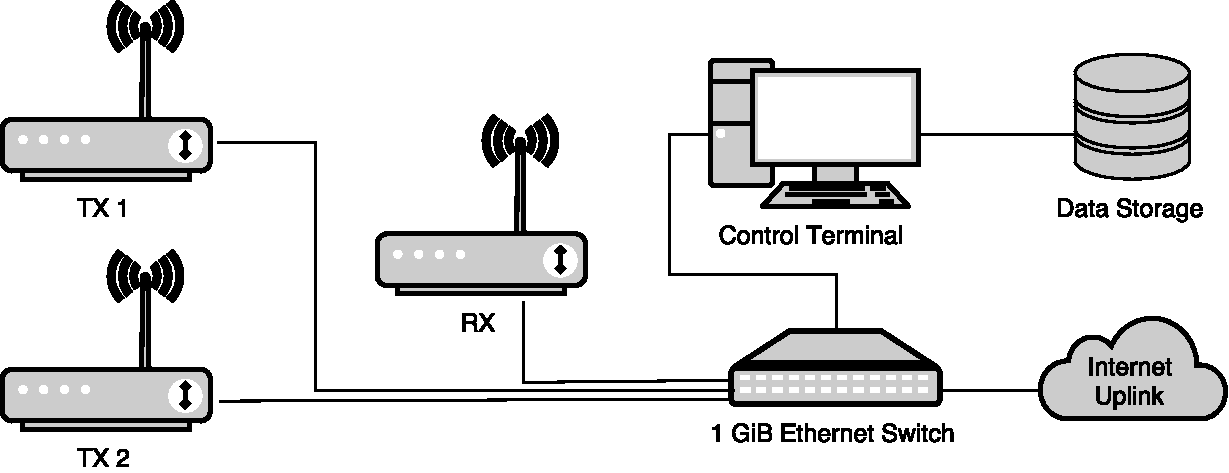
\includegraphics[width=\textwidth]{gfx/images/warp-layout}
	\caption{WARP SDR Experiments Hardware Layout}
	\label{fig:warp-layout}
\end{figure}

The experiments were carried out in a typical office building. This means that there were multiple IEEE 802.11 networks with several dozens of connected clients. I used a standard WLAN channel and no electromagnetic shielding.\\

Since the \gls{WARP} boards use a sampling frequency of 40 MHz, but the Matlab WLAN Systems Toolbox creates time-domain samples with a 20 MHz sampling rate, I used interpolation to adapt frequencies. This is done with the built-in \texttt{resample} Matlab function. Listing \ref{lst:resample} illustrates the process.

\begin{lstlisting}[captionpos=b,caption={Interpolate Sampling Rate},label=lst:resample]
% Interpolate to get from 20 to 40 MHz sampling rate
tx1 = resample(tx1, 40, 20);
\end{lstlisting}

For the real-world experiments, I deliberately caused frame collisions with the same scrambler initialization and destination \gls{MAC} addresses, and used \gls{MCS} 0. This means that in principal everything was the same as for the most basic simulation experiments.

To assess the basic mechanics of receiving collisions with the \glspl{SDR}, I applied cross-correlation to only one \gls{LTF} symbol instead of the \gls{MAC} addresses and plotted the results. They can be seen in figure \ref{fig:warp_preamble_corr}. The collided frames were aligned with some offset for this experiment.

While one group of spikes is a bit lower than the other, it is still easily possible to detect that there is a collision due to the 4 higher and 2 lower spikes caused by the two \glspl{LTF}. The higher level of noise in the begining of the signal are caused by \gls{AGC} in the receiving \gls{SDR}. Since the \gls{MAC} addresses are located further into the signal, and only that part is correlated for sender detection, this noise should be no problem.

\begin{figure}[H]
	\centering
  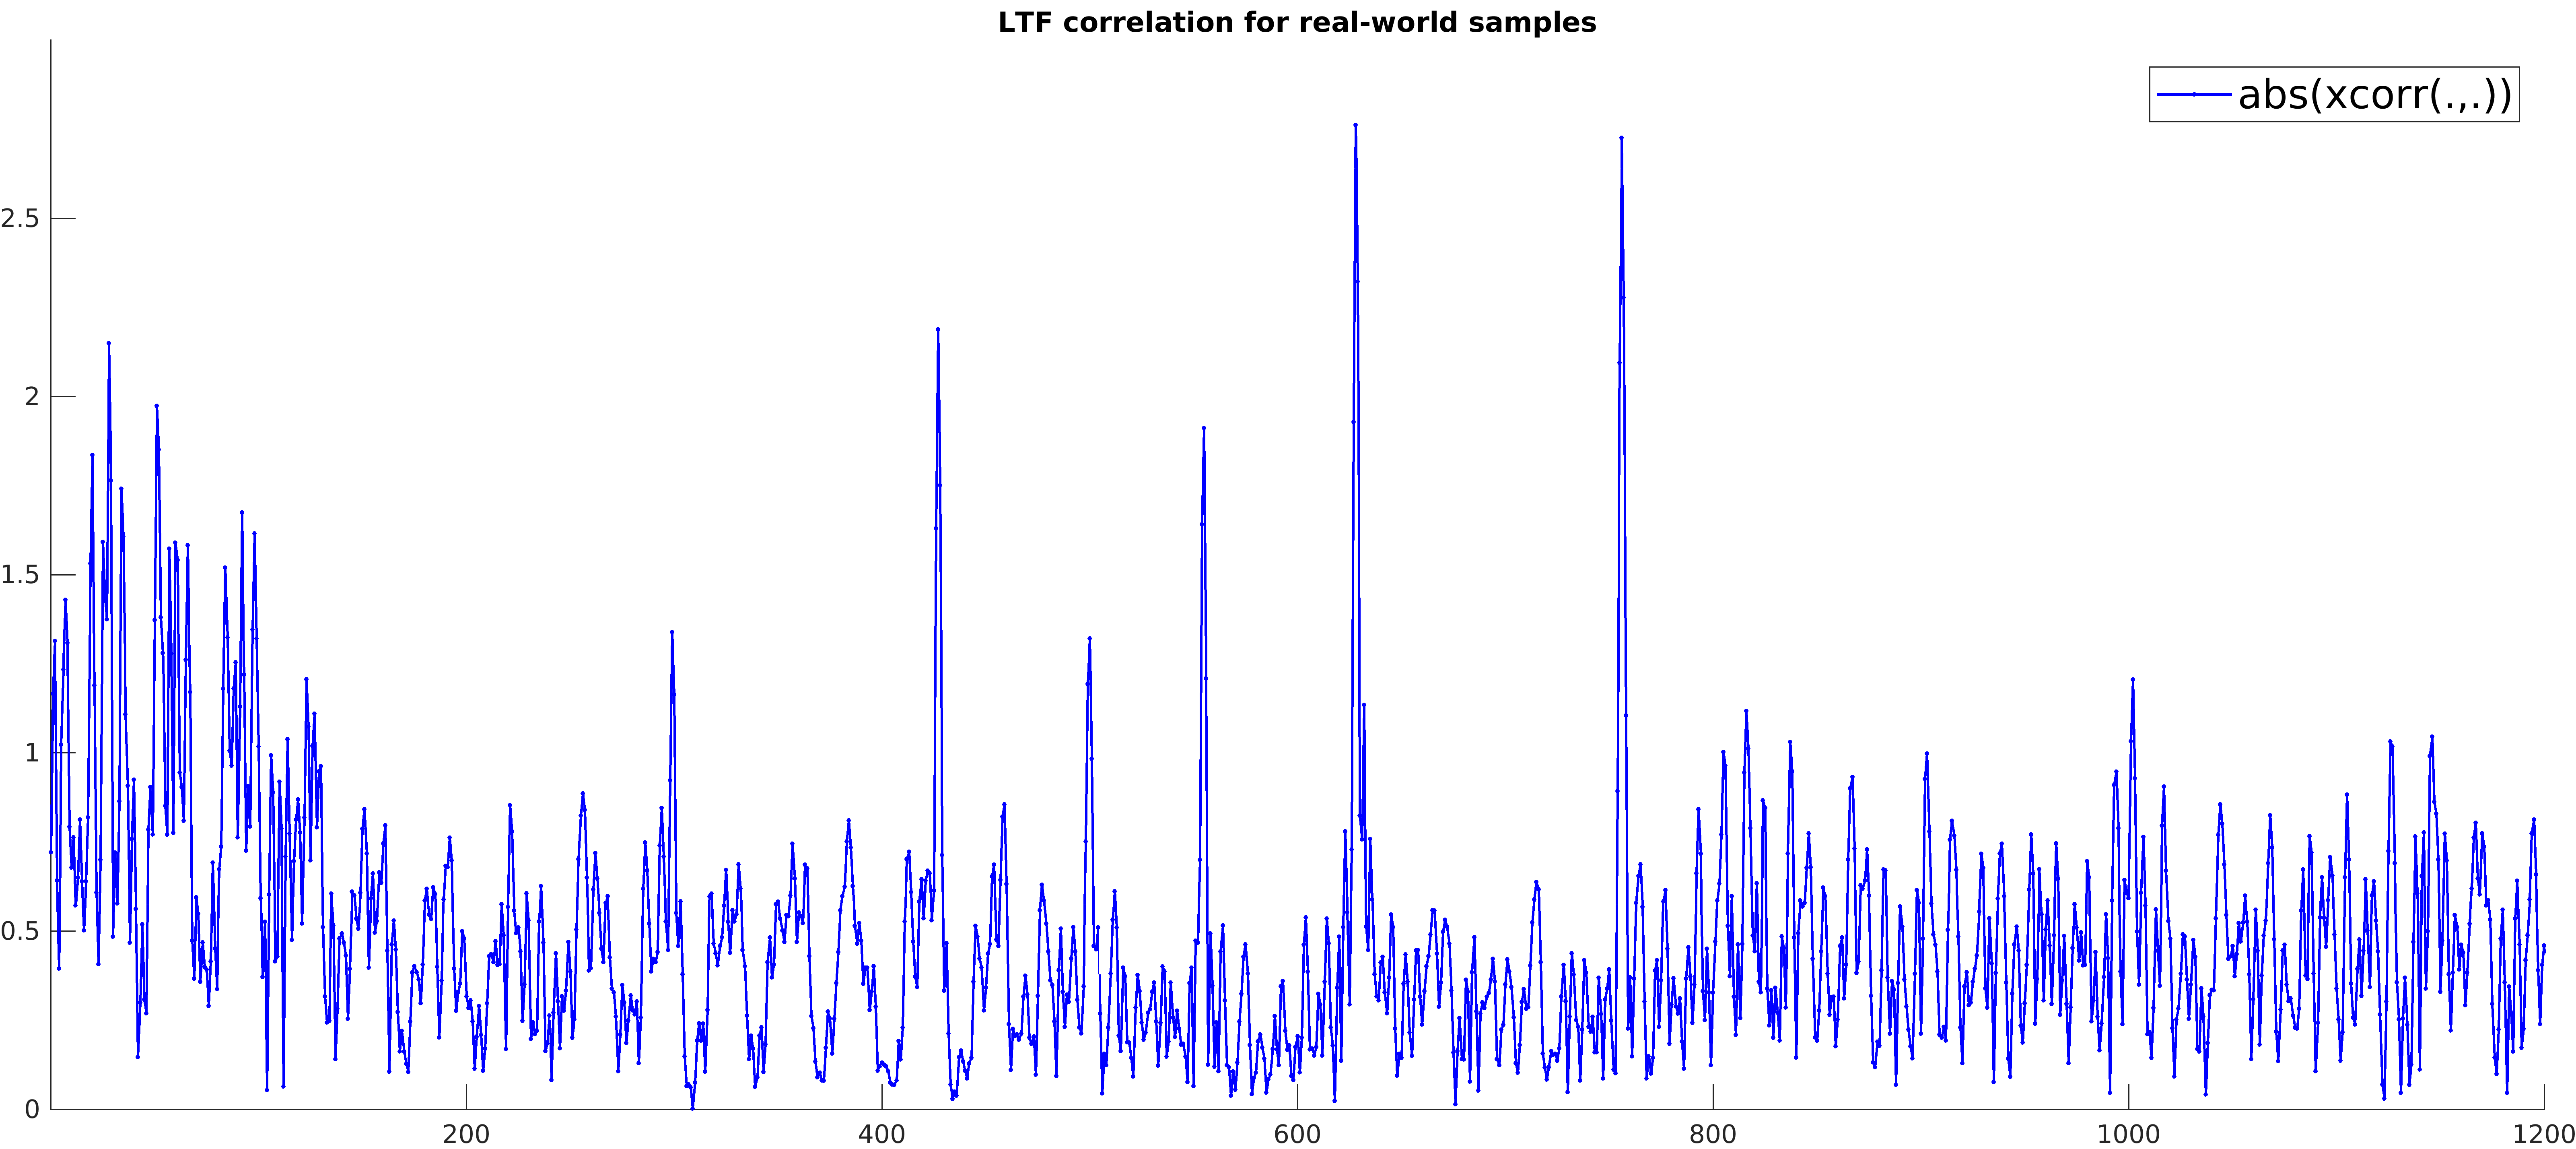
\includegraphics[width=\textwidth]{gfx/plots/capture_collision-20170622-1533-ltf_correlation}
	\caption{Preamble Correlation in WARP Experiment}
	\label{fig:warp_preamble_corr}
\end{figure}

The results of the preamble correlation are promising. They show that indeed a collision of two frames is captured by the receiving \gls{SDR}, and that cross-correlation in the time-domain can in fact tell apart both \glspl{LTF}.

Next, I used the same code as for the simulation experiments to try and detect sender \gls{MAC} addresses. Fortunately, this worked well. In general, the results were very comparable to those of the simulation, however there was a slightly lower accuracy. The reason for that is probably the channel effects, which could not be simulated in full detail by the channel models.

%%% -----------------------------------------------------------------------------

\chapter{Discussion}\label{ch:Discussion}
\glsresetall % Resets all acronyms to not used

This chapter discusses the results of the evaluation, and their implications. Finally, future work is proposed to iterate on the findings.


%% -----------------------------------------------------------------------------

\section{Computational Complexity}\label{sec:complexity}

In order to use the proposed sender detection algorithm, it must be feasible to do all necessary calculations in real-time. In this section, I present an analysis of the computational complexity of the different components.

Two main categories of tasks can be identified. First, the generation of reference signals to use for cross-correlation. This can be pre-computed before any collisions are received and is therefore less time-critical. Second, correlating time-domain samples with the reference signals and sorting to work out a guess which senders participated. This needs to be done for every analyzed collision.\\

Based on the results from the experiments with scrambler initialization and the destination \gls{MAC} address as described in sections \ref{sec:ex-scrambler} and \ref{sec:ex-destination}, the following factors scale up the amount of necessary reference signals:

\begin{itemize}
  \item \gls{MAC} addresses on the network
  \item \glspl{MCS}
  \item Scrambler initialization values
\end{itemize}

The destination \gls{MAC} address can be ignored. This means that the algorithm scales according to the following equation:

$$ N_{\text{RS}} = N_{\text{MAC}} \cdot N_{\text{MCS}} \cdot N_{\text{SI}} = N_{\text{MAC}} \cdot 8 \cdot 127 $$\vspace{0cm}

Here, $ N_{\text{RS}} $ denotes the number of modulated reference signals, $ N_{\text{MCS}} $ is the number of available \glspl{MCS}, and $ N_{\text{SI}} $ describes the amount of possible scrambler initialization values.

Let $ n = N_{\text{MAC}} $ be the number of cached \gls{MAC} addresses on the network. The worst-case asymmetric complexity in this case is:

$$ O(\text{"Sender ~Detection"}) = O(n \cdot 8 \cdot 127) = O(1016 n) = O(n) $$\vspace{0cm}

The algorithm scales linearly with the amount of stations on the IEEE 802.11 network. This is optimal since every station is a possible sender which has to be considered when decoding a collision. It is however debatable whether the linear factor of 1016 is feasible on commodity computing hardware. That would be necessary to enable broad usage of the detection technique across many different devices as mentioned in chapter \ref{ch:introduction}. A quantitative analysis is therefore desirable.\\

I used the Matlab profiler to gather data on the execution speeds of different parts of the algorithm. These measurements were done on a consumer laptop, featuring a 2-core 3rd-generation Intel i3 processor with Hyper-Threading at 1.9 GHz. The results are summarized in table \ref{tbl:timing}.

\begin{table}[ht]
	\centering
	\begin{tabular}{|p{8.5cm}|p{2.5cm}|}
		\hline
		\textbf{Function} & \textbf{Time Spent} \\ \hline
	    wlanTGnChannel & 912 ms \\ \hline
    	wlanNonHTData & 662 ms \\ \hline
	    CRC Calculation & 122 ms \\ \hline
	    awgn & 54 ms \\ \hline
		xcorr & < 1 ms \\ \hline
	\end{tabular}
	\caption{Timing Analysis of the Detecting Algorithm \label{tbl:timing}}
\end{table}

This data suggests that the real-time part of the algorithm, which is limited to cross-correlation with \texttt{xcorr} is negligible when compared to the pre-modulation of reference signals. For small networks, the correlation time is probably fast enough. For high amount of stations however, the complexity gets out of hand quite quickly. For a network with 500 client for example, each collision requires a calculation of about 500 seconds due to the linear scaling factor of 1016. However, it is easily possible to parallelize this workload, or even use specialized hardware such as \glspl{FPGA}. In the extreme case, where every correlation is done at the same time, only 1 ms is needed for decoding the collision.

The calculation of \gls{CRC} checksums is time-consuming, however not needed for the algorithm. Instead, dummy checksums can be used as described in section \ref{sec:matlab-impl}. Therefore, modulation of reference signals scales with the performance of the \texttt{wlanNonHTData} function.

Since the modulation of reference signals can be done ahead of time, the only important case is that of a newly connected client. In this case, 1016 new signals must be created for this new \gls{MAC} address, which takes about 5 minutes without any parallelization. With more CPU cores however, this seems manageable.


%% -----------------------------------------------------------------------------

\section{Detection Quality}\label{sec:detection-quality}

The results of my simulations were very promising. While admittedly only IEEE 802.11 a/g networks were evaluated, as section \ref{sec:mimo} discusses further, detection accuracy was quite high even for higher \glspl{MCS}.\\

In contrast to the scrambler initialization, the value of the preceding destination \gls{MAC} address had hardly any effect on detection quality, as described in section \ref{sec:ex-destination}. Most likely this is because of the relatively small state of the convolutional encoder compared to the size of a \gls{MAC} address. While the encoder considers the last seen seven bits for its output, a \gls{MAC} address comprises 48 bits of data.

Regardless of the preceding destination \gls{MAC} address, the convolutional encoder state is synchronized after the first seven bits of the sender address. This is only a small fraction of about 15 \%. In addition to that, the first seven bits are part of the vendor prefix, which is already to some extent likely to be the same across multiple stations on the network. Therefore, convolutional encoding poses no critical impact on sender detection performance.\\

Using real-world \glspl{SDR}, the detection technique performed reasonably well at least for lower \glspl{MCS}. This is particularly nice because these experiments were conducted in an environment where production wireless traffic was present. Although there was some decrease in detection quality, this shows that the algorithm is capable of successfully recognizing sender \gls{MAC} addresses even when a reasonably high network load is present.


%% -----------------------------------------------------------------------------

\section{IEEE 802.11 n/ac/ax Networks}\label{sec:mimo}

This thesis only covered sender detection for IEEE 802.11 a/g networks. However, such networks are rarely used nowadays due to their low throughput. Modern standards such as IEEE 802.11 n/ac, and the upcoming 802.11 ax are much more relevant.

There are many improvements and differences introduced with the 802.11 n standard. One of the most important with respect to time-domain sample cross-correlation is the adoption of \gls{MIMO} transmission. With this technique, every sender and receiver uses multiple antennas, instead of just one as with 802.11 a/g. This allows for a much higher spectral efficiency, meaning that more bits can be transmitted per used bandwidth \cite{perahia2013}. However, the overall system complexity and multi-path effects in particular make it much more difficult to apply naive time-domain correlation.\\

It would be interesting whether the proposed sender detection algorithm can be adapted to work in a \gls{MIMO} environment. In the current form, this is unfortunately quite unlikely. On the one hand, collision detection and especially the determination of relevant sample periods containing the sender \gls{MAC} addresses must be adjusted to the physical layer high-throughput frame format used by modern standards \cite{ieee2012}.

On the other hand, using multiple streams implies the possibility that the sender \gls{MAC} address gets fragmented. While some bits could be transmitted in the first stream, the remaining bits could be sent in various other streams. This renders simple cross-correlation with \texttt{xcorr} directly on the received sample vector useless.


%% -----------------------------------------------------------------------------

\section{Future Work}

The preceding discussion reveals some serious problems with the proposed algorithm for sender \gls{MAC} address detection. The fundamental principles however do seem promising. There are remaining questions that should be addressed in further research.\\

\textit{Quantitative Noise Evaluation with SDRs}\\

As mentioned in section \ref{sec:detection-quality}, noise from other stations in the network could cause the correlation of \gls{MAC} addresses to degrade. Whether this is the case, and to which extent it influences detection performance, could be evaluated in a quantitative analysis. As a first step, the experiments with \gls{WARP} \glspl{SDR} should be reproduced in a radiation-free environment, such as a Faraday cage. If the technique performs better in that case, additional IEEE 802.11 devices could be added one at a time, continuously measuring the algorithm's accuracy.\\

\textit{MIMO and IEEE 802.11 n/ac/ax}\\

In a next step, the technique could be adapted to current IEEE 802.11 standards, such as 802.11 n/ac. This involves finding a solution to the problems with \gls{MIMO}, as described in section \ref{sec:mimo}, especially the fragmentation of \gls{MAC} address bits onto different spatial transmission streams.\\

\textit{Implementation on Mobile Operating Systems}\\

In order to be used with possible new \glspl{DCF}, it is interesting how the sender detection algorithm performs on mobile operating systems, Android and Apple iOS in particular. Since almost everybody has a smartphone these days, those operating systems power a significant fraction of stations in IEEE 802.11 networks. While desktop operating systems are also very important, mobile platforms face the additional issue that due to limited battery power, calculations are inherently more expensive.

Future work could implement sender detection on collisions as a kernel module for mobile platforms and evaluate its performance and accuracy. A special focus should be set to complexity, power usage, and overall implications on device usability and responsiveness.

%\include{chapters/07-conclusions}


%% ---------------------------------------------------------------------------------------------------------------------

\appendix
%% ---------------------------------------------------------------------------------------------------------------------

\chapter{Appendix}\label{ch:Appendix}

\glsresetall % Resets all acronyms to not used


%% ---------------------------------------------------------------------------------------------------------------------

Start a chapter with text and not with a section header. Open the
\emph{classicthesis-config.tex} file to insert the title of your thesis, the
names of your supervisors and the hand-in date of your thesis.


%% ---------------------------------------------------------------------------------------------------------------------

\section{First Section}
\label{sec:first_section}

After a section there should always be text before the next section. The first
paragraph is always without indentation. Starting from the second paragraph,
there is an indentation.

Here is an equation that you can reference:
\begin{align}
	\underbrace{\begin{pmatrix}\mathcal{B}_1\\\mathcal{B}_2\\\vdots\\\mathcal{B}_R\end{pmatrix}}_\mathcal{B} &= \underbrace{\begin{pmatrix}H_{1,1} & H_{1,2} & \hdots & H_{1,T}\\H_{2,1} & H_{2,2} & \hdots & H_{2,T}\\\vdots & \vdots & \ddots & \vdots\\H_{R,1} & H_{R,2} & \hdots & H_{R,T}\end{pmatrix}}_{H_{A\rightarrow B}}\cdot \underbrace{\begin{pmatrix}\mathcal{A}_1\\\mathcal{A}_2\\\vdots\\\mathcal{A}_T\end{pmatrix}}_\mathcal{A}\label{eqn:example}
\end{align}


\subsection{Referencing}

Take a look in the following list to reference sections, figures and equations:
\begin{itemize}
	\item \autoref{sec:first_section}
	\item \autoref{fig:wiretapchannel}
	\item \autoref{eqn:example}
\end{itemize}


\subsection{Acronyms}
For acronyms you should use the \emph{glossaries} package and put your acronyms
in the \emph{FrontBackmatter/acronyms.tex} file. The first acronym is always
written in it's long form, the following occurrences are abbreviated: first
occurrence \gls{SNR}, second occurrence \gls{SNR}, plural \glspl{SNR}.


\subsection{Examples on Figures}

\sloppy
When using figures, use vector graphics whenever possible. In
\autoref{fig:wiretapchannel} and redacted are some examples to
generate vector graphics directly from \LaTeX code. The second example is based
on the \emph{matlab2tikz} script for matlab. You find an example in the
\mbox{\emph{gfx/matlab/create\_example\_graph.m}} file. TikZ is used to generate
the graphics. As it takes some time and memory to recompile a graphic, pdflatex
caches generated figures when the \lstinline|--enable-write18| switch is set
when calling \lstinline|pdflatex|. Graphics are only recompiled when you
uncomment the \lstinline|\tikzset{external/remake next}| command. Figures should
always appear after the first reference in the text or at the top of the same
page as the reference, but never before the reference. Prefer placing figures on
separate pages. Try to always have figures and text on each page. Or place
enough figures to fill a page only with figures.

\begin{figure}
	\centering
	\begin{tikzpicture}[node distance=6mm]
	\node[dspsquare,minimum height=3.2em, minimum width=5em,text height=1em, fill=white]
	(source) {Source};
	\node[dspsquare,minimum height=3.2em, minimum width=5em,text height=1em, fill=white, right=of source]
	(encoder) {Encoder};
	\node[dspsquare,minimum height=3.2em, minimum width=7em,text height=2em, fill=white, right=of encoder]
	(mainch) {Main Channel\\$Q_M$};
	\node[dspnodefull, right=of mainch] (n1) {};
	\node[dspsquare,minimum height=3.2em, minimum width=5em,text height=1em, fill=white, right=of n1]
	(decoder) {Decoder};
	\node[coordinate,right=of decoder] (n2) {};
	\node[dspsquare,minimum height=3.2em, minimum width=10em,text height=2em, fill=white, below=1cm of n1]
	(wiretapch) {Wiretap Channel\\$Q_W$};
	\node[coordinate,below=of wiretapch] (n3) {};

	\draw[dspconn] (source) -- node[midway,above] {$S^K$} (encoder);
	\draw[dspconn] (encoder) -- node[midway,above] {$X^N$} (mainch);
	\draw[dspconn] (mainch) -- node[midway,above] {$Y^N$} (decoder);
	\draw[dspconn] (decoder) -- node[midway,above] {$S^K$} (n2);
	\draw[dspconn] (n1) -- (wiretapch);
	\draw[dspconn] (wiretapch) -- (n3) node[below] {$Z^N$};
	\end{tikzpicture}
	\caption[The wiretap channel]{The wiretap channel (source: redacted)}
	\label{fig:wiretapchannel}
\end{figure}


%% ---------------------------------------------------------------------------------------------------------------------

\section{Margin Notes}

Especially in the standard SEEMOO template with wide margins, you are
\marginpar{Here you can add text to the margin. For example, to
	summarize the section next to it.} encouraged to insert text into the
margins. If you decide to do so, plan to have at least one margin note
per double page.



%% ---------------------------------------------------------------------------------------------------------------------

\cleardoublepage%% ---------------------------------------------------------------------------------------------------------------------
% Bibliography


% work-around to have small caps also here in the headline
\manualmark
\markboth{\spacedlowsmallcaps{\bibname}}{\spacedlowsmallcaps{\bibname}} % work-around to have small caps also
%\phantomsection 
\refstepcounter{dummy}
\addtocontents{toc}{\protect\vspace{\beforebibskip}} % to have the bib a bit from the rest in the toc
\addcontentsline{toc}{chapter}{\tocEntry{\bibname}}
\label{app:bibliography}
\printbibliography

\cleardoublepage%% ---------------------------------------------------------------------------------------------------------------------
%  Declaration


%\refstepcounter{dummy}
%\pdfbookmark[0]{Thesis Statement}{statement} \chapter*{Thesis Statement}
%\thispagestyle{empty}
%\begingroup
%\let\cleardoublepage\relax
%\begin{flushright}
%	\emph{pursuant to §\,22 paragraph 7 of APB TU Darmstadt}
%\end{flushright}
%I herewith formally declare that I have written the submitted \myDegree{} independently. I did not use any outside support except for the quoted literature and other sources mentioned in the paper. I clearly marked and separately listed all of the literature and all of the other sources which I employed when producing this academic work, either literally or in content. This thesis has not been handed in or published before in the same or similar form.
%In the submitted thesis the written copies and the electronic version are identical in content.
%
%\bigskip
%
%\noindent\textit{\myLocation, \myTime}
%
%\smallskip
%
%\begin{flushright}
%	\begin{tabular}{m{5cm}}
%		\\ \hline
%		\centering\myName \\
%	\end{tabular}
%\end{flushright}
%
%\vfill

\selectlanguage{ngerman}
\pdfbookmark[0]{Erklärung zur Abschlussarbeit}{erklaerung} \chapter*{Erklärung zur Abschlussarbeit}
\begin{flushright}
	\emph{gemäß §\,22 Abs.\,7 APB der TU Darmstadt}
\end{flushright}
Hiermit versichere ich, \myName{}, die vorliegende \myDegree{} ohne Hilfe Dritter und nur mit den angegebenen Quellen und Hilfsmitteln angefertigt zu haben. Alle Stellen, die Quellen entnommen wurden, sind als solche kenntlich gemacht worden. Diese Arbeit hat in gleicher oder ähnlicher Form noch keiner Prüfungsbehörde vorgelegen.

Mir ist bekannt, dass im Falle eines Plagiats (§38 Abs.2 APB) ein Täuschungsversuch vorliegt, der dazu führt, dass die Arbeit mit 5,0 bewertet und damit ein Prüfungsversuch verbraucht wird. Abschlussarbeiten dürfen nur einmal wiederholt werden.

Bei der abgegebenen Thesis stimmen die schriftliche und die zur Archivierung eingereichte elektronische Fassung überein.

\bigskip

\noindent\textit{\myLocation, \myTime}

\smallskip

\begin{flushright}
    \begin{tabular}{m{5cm}}
        \\ \hline
        \centering\myName \\
    \end{tabular}
\end{flushright}

\selectlanguage{american}



\end{document}

